\documentclass{acm_proc_article-sp}
\usepackage{url}

\begin{document}

\title{Framing-Based Camera Tool for Artists\\in Game Development}

\numberofauthors{4}
\author{
% 1st. author
\alignauthor
Mathias K. Berthelsen\\
       %\affaddr{Aalborg University, Denmark}\\
       \email{mkbe11@student.aau.dk}
% 2nd. author
\alignauthor
Gustav Dahl\\
       %\affaddr{Aalborg University, Denmark}\\
       \email{gdahl11@student.aau.dk}
% 3rd. author
\and
\alignauthor
Benjamin N. Overgaard\\
       %\affaddr{Aalborg University, Denmark}\\
       \email{boverg11@student.aau.dk}
  % use '\and' if you need 'another row' of author names
% 4th. author
\alignauthor
Andreas M. Thomsen\\
       %\affaddr{Aalborg University, Denmark}\\
       \email{amth11@student.aau.dk}
}

\maketitle

\begin{abstract}
The framing-based camera tool (FCT) is a tool for games where the player character moves on a pre-defined path. Through participatory methods, it was found that artists prefer working with keyframing animation, known from traditional time-based animation. This concept has been incorporated in the FCT in the form of framings. A framing consists of a an influence point and a camera. Depending on where the player is located, the main camera will interpolate between the framings.

(not finished)

%(from Kraus): a tool for artists to define an interactively moving camera in a game where the player avatar can only move along predefined paths

% feedback from Kraus:
We should do:
Importance of cam in games
Difficulties of artists using
We present ... we do this
Time-based animation ???

\end{abstract}

% A category with the (minimum) three required fields
%\category{H.4}{Information Systems Applications}{Miscellaneous}
%A category including the fourth, optional field follows...
%\category{D.2.8}{Software Engineering}{Metrics}[complexity measures, performance measures]

\terms{Game development}

\keywords{Game development, camera system, AI, interpolation, workflow, participatry design, collaboration} % NOT required for Proceedings

\section{Introduction}
%BASED ON PRELIMIANARY RESEARCH, TOOLS SHOULD BE DEVELOPED WITH A MODULAR MINDSET AND ALLOW FOR TWEAKABLE PARAMTERS and stuff

%Describe basic concept of the product (context)
%We have a collaboration with TAW
%They make 3D point n click game
%Framing system
%Path system
\textbf{real world problem}
\textbf{Time based > interactive}
\textbf{Gap of knowledge}
\textbf{Opgaver / features er unclear, derfor bruger vi PD}

ANDREAS

This project is based on a collaboration between Medialogy and a group of artists from The Animation Workshop (TAW) in Viborg. As their bachelor project, the students at TAW developed a 3D point 'n click game, \textit{FEELS}, for the iPad using the Unity game engine. The TAW project spanned two semesters (pre-production and production), whereas this Medialogy project lasted only the first semester. Two additional programmers have also been working full-time on the project.

During the collaboration, it was decided that we should focus on developing a camera system for the game. This tool should empower the artists, so that the artists didn't have to worry about technical details. It should be simple to set up and function in a similar fashion as other 3D applications that the TAW students have been trained in during their three-year education. The camera tool was chosen, since it does not directly influence and interfere with the gameplay, making it easier for the other programmers to work directly on the game.

Before we began designing and implementing the tool, we conducted several preliminary studies to get an understanding of how game development tools should be made. We visited two game companies (KnapNok Games and Unity Studios), as well as conducting an online survey to gather, information about game development tools. The key findings were that the tool should be developed in a modular fashion and allow the user to tweak as many parameters as deemed necessary. Additional notes from the studies can be found in \textbf{APPENDIX X}.


There are many ways to design camera motions in games. Fundamentally, one can distinguish between \textit{cinematic sequences} and \textit{interactive gameplay}. These two are typically considered mutually exclusive, because cinematic sequences per definition is non-interactive \cite{haigh-hutchinson_real-time_2009}. However, it is also possible to mix those two, so the camera can dynamically adapt to certain things happening in the game, e.g., game events and player input. This means that a sequence does not have to be viewed in exactly the same way every time. For example, depending on the player's movement, the camera can change accordingly.

%Sometimes it might be necessary to put certain restrictions on where the player can move. An example of this could be a special "boss battle" where the player is confined in a restricted area. Typically, the camera would zoom out and focus on specific parts of this boss enemy (e.g. a weak point). The camera dynamically frames the scene in such a way so that the player and the enemy are visible at all times \cite{haigh-hutchinson_real-time_2009}.

Games often require the ability to replay previous sequences of the gameplay. This can be used to replicate certain events to re-create the motion and visual state of objects in a scene \cite{haigh-hutchinson_real-time_2009}. It can be achieved by recording the rendering state of objects on a set amount of frames, and then use \textit{interpolation} to calculate the state of said objects. Interpolation is a method of inserting intermediate values into a set of data and makes it possible to take sampled data and generate new points in between \cite{haigh-hutchinson_real-time_2009}. Replaying of this data can be referred to as \textit{keyframing}. Keyframing of camera data requires position and orientation of the camera, together with a time interval between the samples \cite{haigh-hutchinson_real-time_2009}.
\section{Related Work}\label{relatedWork}
%Camera Path Animator 3.0 (Unity asset store).
%Camera system that follows the character but also focuses on showing the environment - Used in the game God of War.

\begin{figure*}[htbp]
\centering
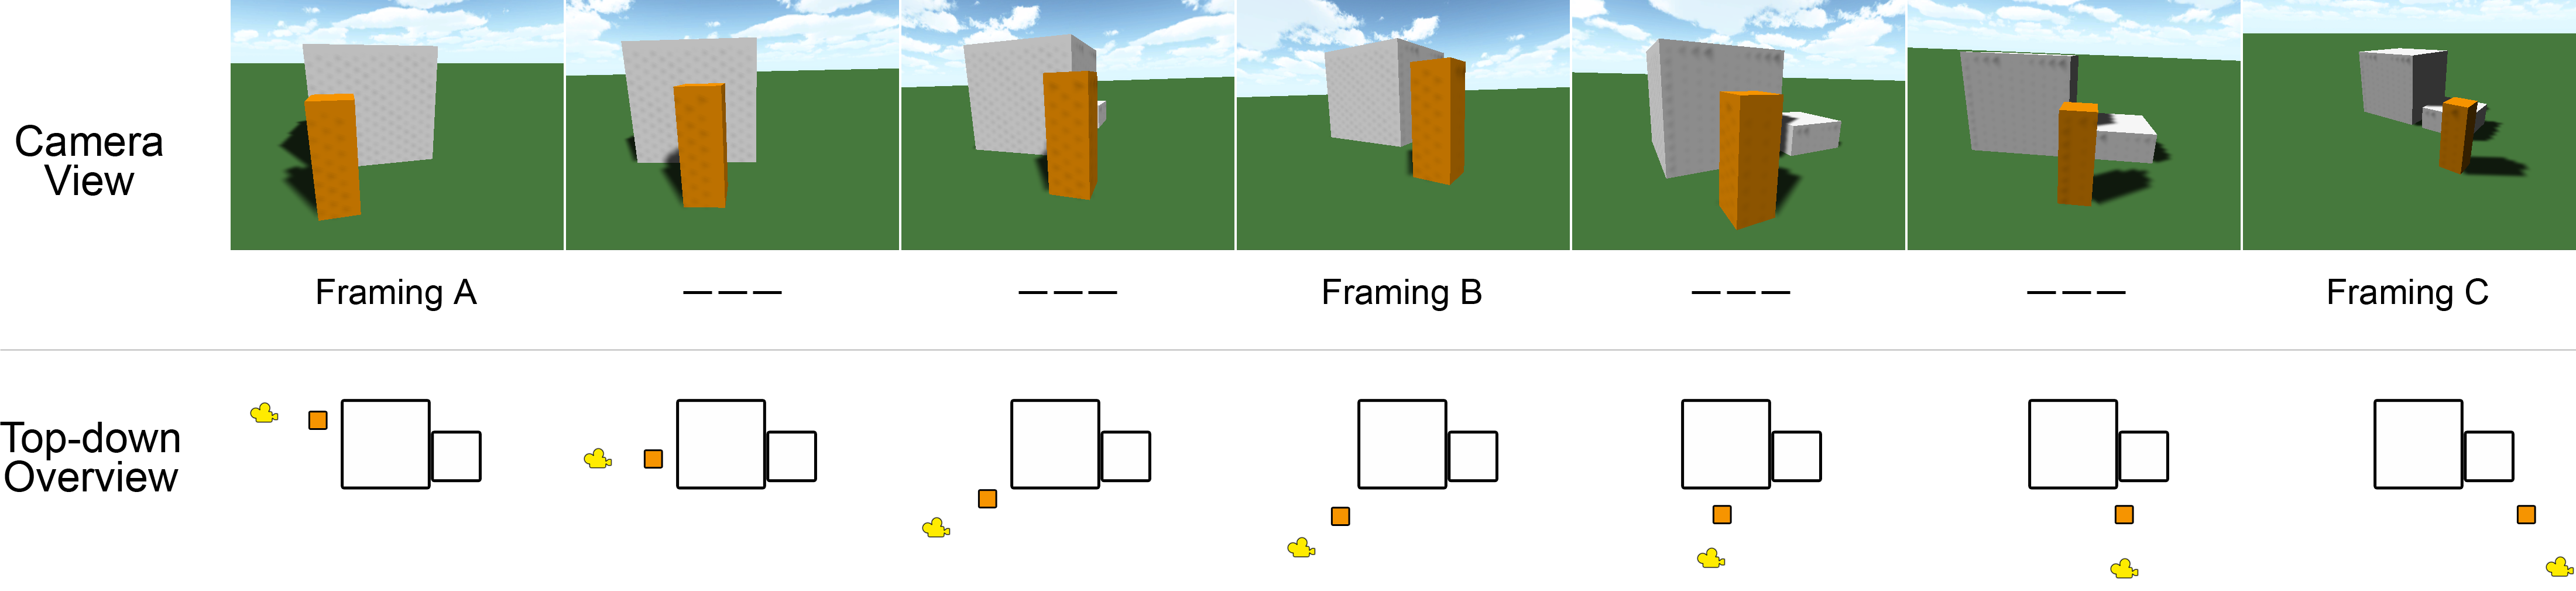
\includegraphics[width=1\textwidth]{Pics/InterpolationExample}
\caption{An example of a camera interpolation between three framings (A, B and C). The framings contain position, rotation and field of view. As the player character (orange cube) moves, the camera follows him by interpolating between the framings.}
\label{fig:InterpolationExample}
\end{figure*}

Automatic camera control is an active research field. In 3D computer animation, a virtual environment is rendered in frames from a specific point of view. This is a complex process that involves technical and artistic tasks, typically requiring the work of several professionals for a long time period \cite{burelli_automatic_2014}. Developing a system that makes the camera animation automatic can be beneficial at both a professional level (to reduce cost) or at an amateur level (to increase quality). Systems that emphasize automatic behaviour have been proposed \cite{bourne_constraintBased_2008, burelli_automatic_2014}; these use an automatic approach for controlling a virtual camera driven by AI techniques. However, the focus of the camera tool proposed in this work is on artistic control. Hence, an automatic approach is not feasible.

In a behind-the-scenes documentary, the developers behind the PlayStation game series \textit{God of War} talk about the importance of being able to frame the scene \cite{gow_camera}. Depending on the context, it is important for them to frame the scene so players know where they should be heading next. They use camera zones to determine what area the player is in and then activate the corresponding camera for that zone. This example shows that it is important that the artists are able to crate framings themselves.

The main requirement of a framing-based camera tool for games is that it can go from one camera setting (A) to another camera setting (B) depending on the player's position or certain events. For instance, A and B can be different in position, rotation and field of view.
%By looking at games with emphasis on its visuals and environments, it was found that the camera changes its position, rotation and field of view. 
Figure \ref{fig:InterpolationExample} shows an example of how the camera interpolates between three positions.

%\begin{figure}[htbp]
%\centering
%
\includegraphics[width=.4\textwidth]{Pics/CameraSystem_BASIC}
%\caption{The camera interpolates between position A and B. A and B contain information about its %position, rotation and field of view.}
%\label{fig:CameraSystem_BASIC}
%\end{figure}

%\subsection{Camera Tools}
The tool Camera Path Animator \cite{unity_camTool} can be used for creating animated cameras within the game engine Unity \cite{unity_main}. As the name suggests, it works by animating the camera along a specified path, which can have various shapes (e.g., Bezier and Hermite curves). The tool is primarily targeted towards creating cameras that move linearly along a set path, i.e., for use in cinematic sequences. It provides various ways of inserting, moving and deleting points, as well as changing settings such as field of view, speed, interpolation type and easing. Additionally, it has an event system for triggering certain events at certain points in the path. For our tool, it was important that the artists can create framings themselves and that the interface in general is designed for the artists; hence, we chose not to extend the Camera Path Animator, but instead took inspiration from it.

%Why we don't use Camera Path Animator:
%Customizable interface
%Specific for artists
%Freedom
%Flexibility
%Maya knowledge
%Path

%\begin{figure}[htbp]
%\centering
%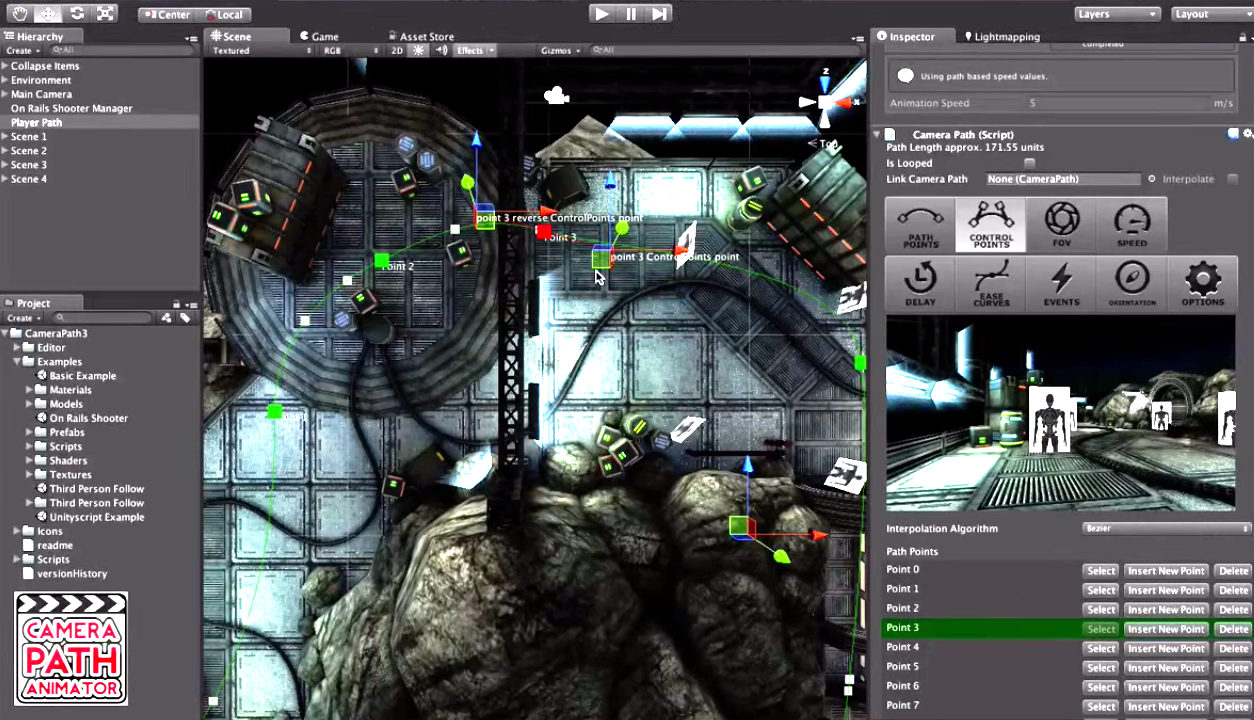
\includegraphics[width=0.40\textwidth]{Pics/unity_path_cam_tool}
%\caption{Overview of the objects related to the camera system.}
%\label{fig:unity_path_cam_tool}
%\end{figure}

%The God of War video game franchise for the PlayStation systems has also made notable use of their camera systems. The developers call the system Rail Driven Cameras and consists of a 'rail' that will be placed in the game world. A camera is keyed in both ends of the rail, and the camera will then animate between them as the protagonist moves along the rail. % Det her føles pølse, ikke meget at skrive om det og super unscientific

%\begin{figure}[htbp]
%\centering
%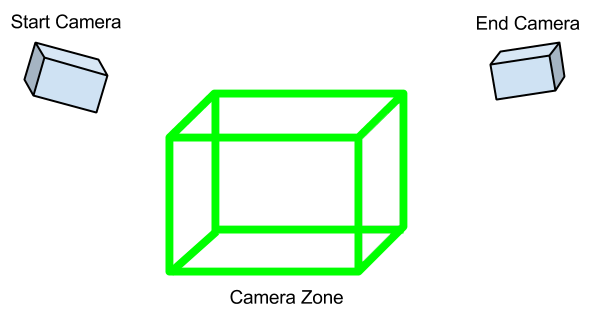
\includegraphics[width=0.45\textwidth]{Pics/gow_cameraZones2}
%\caption{When the player enters a camera zone, the camera will interpolate between the two pre-%defined cameras associated with that zone.}
%\lab%el{fig:gow_zones}
%\end{figure}

%\begin{figure}[htbp]
%\centering
%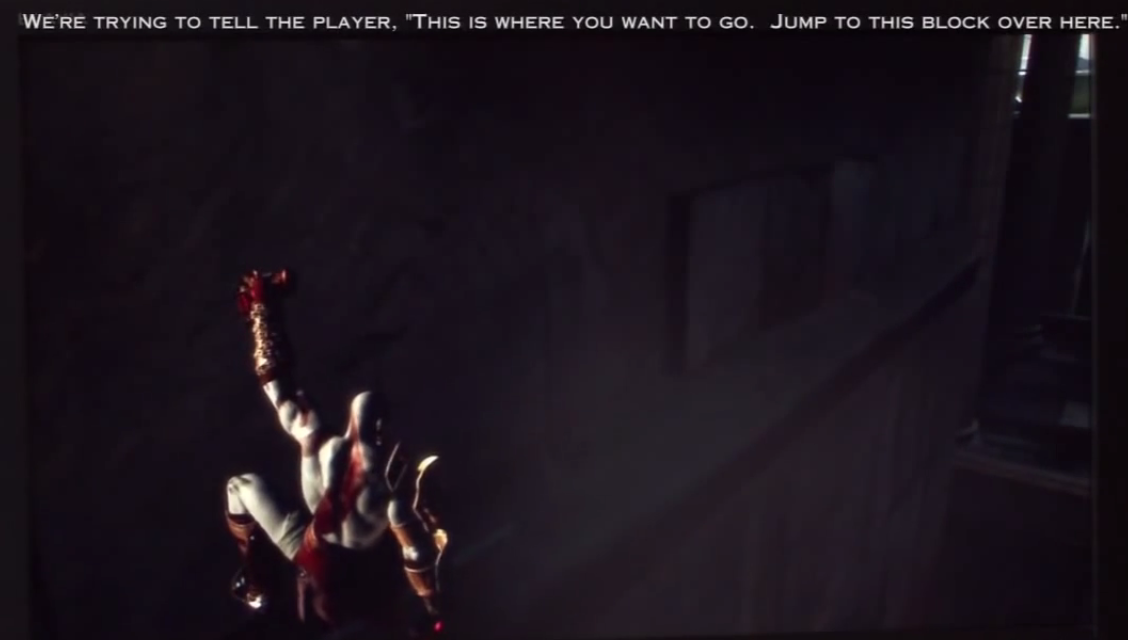
\includegraphics[width=0.40\textwidth]{Pics/gow_next}
%\caption{The camera's framing can help the designer guide the player in the right direction.}
%\label{fig:gow_jump}
%\end{figure}


%An example of this is when the main character has to jump from one 



%\textbf{Scientific material: Write about automatic camera tools (Paulo something-something) - even though we are not using it. Make it clear that our work is different from how other people's camera tools work}

%\subsection{Participatory Design}
Participatory design has been defined as the participation of users in the design process of a system that is to be implemented in an organization \cite{kensing_participatory_1998}. By involving users in the design, their skills, experiences, and interests are taken into consideration, thereby increasing the likelihood that the system will be useful to them.

According to participatory design researchers, it is important that there is an active cooperation between the designer and the user \cite{kensing_participatory_1998}. This results in the designer gaining knowledge of the user's current work practices, and the user gaining knowledge of the technology being developed. It is also important that users take an active part in the analysis of needs, selection of technology, design and prototyping, as well as organizational implementation.
\section{Participatory Design Findings}
The user group of the tool is a team of six third year students from The Animation Workshop in Viborg, Denmark who are developing a 3D point-and-click adventure game \textbf{(INSERT REFERENCE TO GAME GENRE)}.  The team is a mixture of students from two different educations at the school; Computer Animation and Computer Graphics \textbf{(INSERT REFERENCE TO TAW WEBSITE)}. The students will from here on be referred to as artists.  All artists are familiar with making animation films with Autodesk Maya, however it is the first time they are making a video game. Since the start of the project, the students have been educated in working with the Unity game engine.
A requirement for the camera tool as requested by the team, was that it should work with a path system, which is used for player navigation. Furthermore, it was requested that the camera should give the artists the freedom to frame the scene as they want, in order to focus on different elements in the scene.
To create a tool that takes the artists' current skills and experience into consideration, thereby easing their learning curve, techniques from participatory design were used.

\subsection{Participatory Design Activities}
Four different activities using a combination of participatory design techniques were conducted with four artists from the team who had an interest in working with the camera tool. All activities were combined with open interviews as well as video recorded for further analysis.

The first activity, was an observation (INSERT REFERENCE) of the artists working in Maya and Unity. The artists were asked to think-aloud (INSERT REFERENCE) while performing simple tasks relevant to camera work in Maya and Unity. The purpose of this activity was to gain firsthand experience with the artists' current work practices in Maya as well an understanding of how familiar they were with Unity. The activity took 10-15 minutes per person.

Second, the artists were asked to list and sketch the features that they would like to see the most in the camera tool. This activity took inspiration from the 'Freehand Drawing' technique (INSERT REFERENCE). The purpose of the activity was to get a foundation for which tasks the artists wanted to be able to do. The activity took 10-15 minutes per person.   

After sketching, the artists were asked to visualize the interface of the camera tool by arranging a set of pre-made buttons and windows out of paper based on Unity's interface. The activity took inspiration from the 'Collage' technique (INSERT REFERENCE) and its purpose was to get a foundation for the interface design. This activity took 10-15 minutes per person.

The final activity was made after the first design iteration...

\subsection{Findings}
Through the participatory design exercises, we found that the artists were very familiar with Autodesk Maya \cite{MayaSource}. To ease the learning curve, we decided to design the tool with the overall structure of Maya in mind. This doesn't mean that the tool should directly copy how Maya looks and works, but that, when designing the camera tool, we should keep their established mental models \cite{mentalModels} in mind. Since the artists have been working with Maya and other 3D modelling software, they have a certain understanding and expectation of the animation process. As a designer, you create conceptual models for the system. Therefore, it's important to be aware of the users' pre-existing mental models. Another key finding was the fact that most of the artists were working with two computer monitors. This enables them to have the main interface on one monitor, while the other can show secondary windows such as graph editors or an additional preview window showing the camera's point of view.
\section{Framing-based Camera Tool (FCT)}
\subsection{Framing Concept}
In traditional animation, keyframes correspond to a point in time, meaning that when the animation reaches this point in time, the values of this particular keyframing are dominating. Usually, this means that in between keyframes some interpolation is happening. 

%This interpolation is per default linear, but can be manipulated in a graph editor. Anything that can be represented by numbers can be manipulated through keyframes.

Since games don't follow a linear structure like a movie, keyframes can't be associated with a point in time, . In this game, the player is able to move freely around within a pre-defined path. FCT is designed with the player's position in mind. Instead of associating keyframes with time, they are associated with positions in the game's world.

%The game is path-based, which means that the player can only walk on a pre-defined path.

To avoid confusion with traditional keyframing, ours have been dubbed \textit{framings}. A framing consists of an \textit{influence point} and a \textit{camera} (see Figure \ref{fig:framingConceptNew}). The camera holds all of the camera features, such as position and rotation of the camera, as well as field of view. The influence point only has a position. When the player's position is the same as an influence point, the associated camera will dominate. This means that the main camera will use the settings of this camera. Moving between influence points causes an interpolation between each associated camera. Additionally, the interpolation can be manipulated in a graph editor.

\begin{figure}[htbp]
\centering
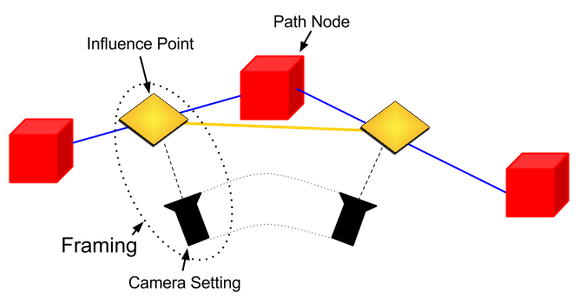
\includegraphics[width=0.4\textwidth]{Pics/Instructions}
\caption{Illustration of the framing concept. A framing consists of an influence point and a camera.}
\label{fig:framingConceptNew}
\end{figure}

\subsection{Path System}
The game is based on pre-defined paths that the player can walk along.
\textbf{MATHIAS/BENJAMIN, SKRIV NOGET HER!}

\subsection{Placing an Influence Point}
After a path has been defined, framings can be placed along this path using the mouse. To indicate that an influence point is going to be created, a small diamond-shaped icon appears near the cursor (see Figure \ref{fig:placingInfluencePoint}). This point snaps to the path. Since the player can only work on the path, it is impossible to create an influence point outside of the path. When clicking with the mouse on the path, the system creates a framing. The connection between an influence point and camera is indicated by a small line. The influence point and the camera can be moved and adjusted independently.

Creating a framing while having another framing selected connects the two. This connection is needed for manipulating the interpolation. The interpolation can be adjusted using the built-in graph editor in Unity (see Figure \ref{fig:curve}).

\begin{figure}[htbp]
\centering
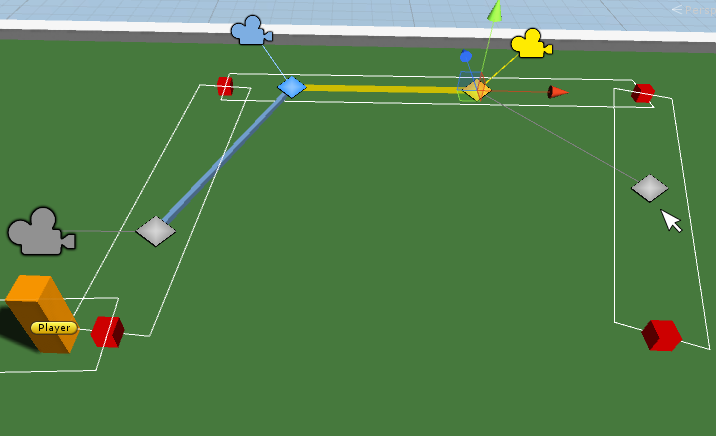
\includegraphics[width=0.45\textwidth]{Pics/placingInfluencePoint}
\caption{You place influence points by holding down the CTRL key and clicking with mouse. These snap to the path defined by the red cubes.}
\label{fig:placingInfluencePoint}
\end{figure}

%Additionally, it is possible to create multiple framings and connect them to each other. This is achieved by selecting an already-created influence point and then clicking to create a new one besides it.

Since the influence point and camera constitutes a framing, the system has been designed so selecting either one selects the framing; hence both provide the same options in the settings window.

\begin{figure}[htbp]
\centering
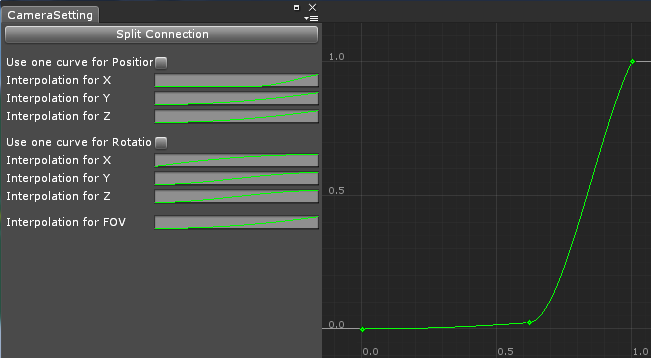
\includegraphics[width=0.4\textwidth]{Pics/curve}
\caption{The graph editor can adjust the interpolation.}
\label{fig:curve}
\end{figure}
\subsection{Adjusting a Camera}
%In Maya, there are multiple ways to accomplish the same thing. An example of this is how to adjust a camera in the scene. This can be done by manually adjusting the X, Y and Z position and rotation of the camera; moving it by dragging a handle tool; or, alternatively, by using the the \textit{Look Through Selected} feature \cite{maya_lookThrough}. During the initial observations, it was clear that many of the artists at The Animation Workshop preferred the latter. This concept was translated directly into the camera tool. Using the \textit{be the camera} feature (see Figure \ref{fig:beTheCam}), the artists can place their camera by navigating the scene in Unity with the \textit{Flythrough mode} \cite{unity_flyMode}.

Besides the traditional ways of aligning objects in Unity (either manually changing X, Y and Z coordinates or adjusting an object via handle gizmos), FCT provides three additional ways: \textit{be the camera}, \textit{snapshot} and \textit{aim point}. The first two take advantage of the scene view in Unity where it is possible to control the camera in a similar way as in first-person controlled computer games. This feature is called the \textit{flythrough mode} \cite{unity_flyMode}. When clicking the \textit{be the camera} button, the tool enters a special mode where the active camera object is automatically aligned to the scene view camera. This means that whatever is visible in the scene view will also be visible by the framing camera. The feature will continue to be enabled until the user exits by pressing the \textit{exit the camera} button. Figure \ref{fig:beTheCam} illustrates this concept. \textit{Snapshot} provides a similar feature, but whereas \textit{be the camera} is continuously activated, \textit{snapshot} only happens one time when the button is pressed.

\begin{figure*}[htbp]
\centering
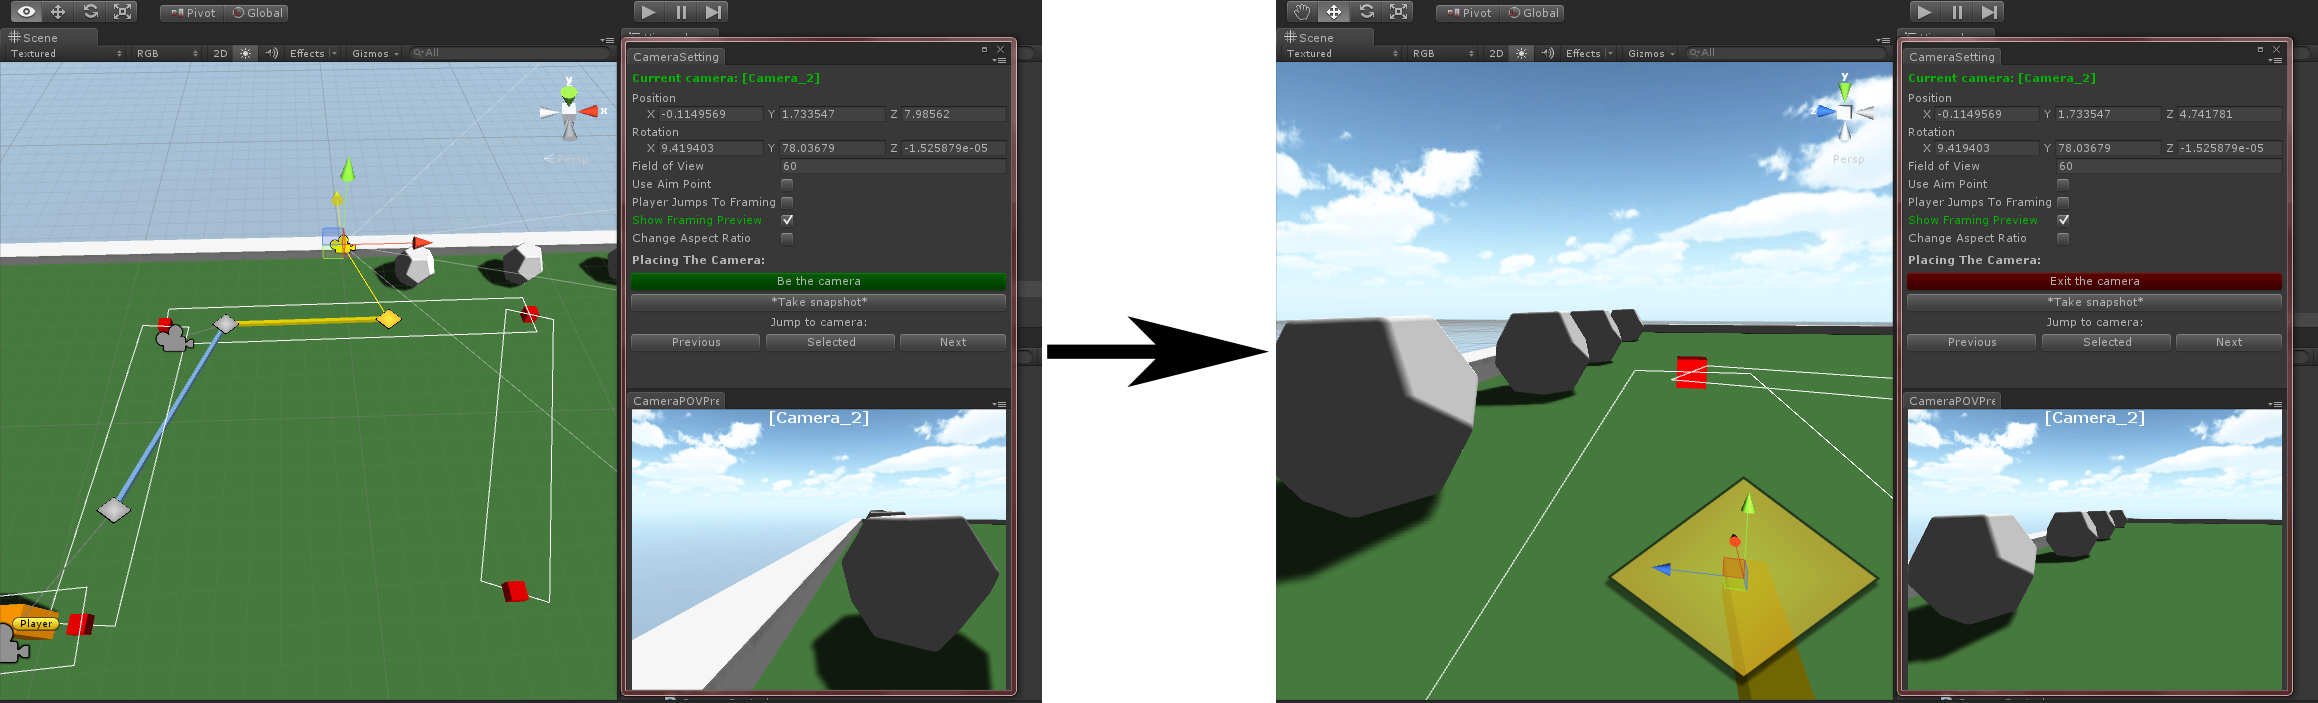
\includegraphics[width=1\textwidth]{Pics/beTheCam}
\caption{Pressing the green button puts the user in a special mode where the selected camera inherits position and orientation data from the scene camera. Notice that only a single rock is visible in the left image. The right image shows how the camera can be moved with the \textit{be the camera} feature to reveal more rocks. The preview image with the [Camera\textunderscore 2] label is how it will look in the actual game.}
\label{fig:beTheCam}
\end{figure*}

A different approach to adjust the camera is by aiming it. This is done with the \textit{aim point}. As the name suggests, the camera will automatically look at this point. This can be used to quickly point at a specific object in the scene, instead of changing the rotation by hand (see Figure \ref{fig:aimPoint}).

\begin{figure}[htbp]
\centering
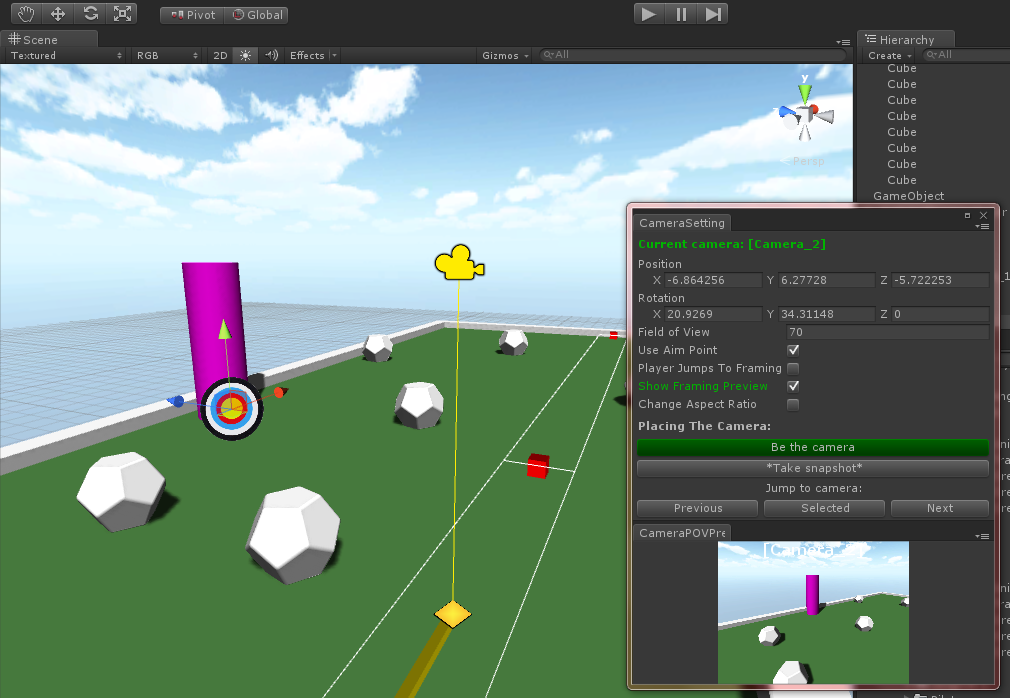
\includegraphics[width=0.4\textwidth]{Pics/aimPoint}
\caption{The aim point (located near the purple cylinder) allows for quick adjustments of the camera.}
\label{fig:aimPoint}
\end{figure}

%It was discovered that none of the artists knew how to use a standard Unity feature that lets the player fly around with the scene camera as if they were playing a first-person game ("Flythrough Mode", \cite{unity_flyMode}). The artist were excited about the discovery of this feature. One artist perceived the standard way of moving around in Unity as confusing, while another stated that the way of moving the camera is exactly like in Maya. After testing this ourselves, we concluded that the movement controls in Maya and Unity are indeed very similar (except for the "Flythrough Mode"), which means that the artists should ideally be comfortable with navigating in either of the applications.

\subsection{Previewing the Interpolations}
FCT provides two ways of previewing the interpolations. One way is to drag the player object around along the path via the \textit{interactive preview}. A different way is to use the \textit{slider preview}. Here, it is possible for the user to select a start framing and end framing and then drag a slider back and forth, changing the interpolation. This provides a quick way to get a feeling of how the camera will interpolate between the framings. Additionally, a "play" button can be pressed to play the interpolation with the actual player velocity (see Figure \ref{fig:slider}).

%The drawback of this method is that you have to manually locate and move the player around in the scene view, which can sometimes be cumbersome.

%An important aspect for the tool was to provide clear feedback.
%A common request from all of the artists were the ability to quickly preview their changes. Instead of having to start the game and navigate the player character to a specific framing, the artists wanted to quickly jump to a specific framing to test out how it feels and looks.

%The artists suggested that they should be able to move the player character around in the editor. Initially, this seemed like a fine way to preview the framings. We did design this feature, but deemed it a bit impractical, since it sometimes would be hard to locate the player character in a big scene. Instead, we took inspiration from Camera Path Animator 3.0 mentioned in Section \ref{relatedWork} by designing an interactive slider. With this feature, the artists are able to choose the start and end framing and interpolate between these. By dragging the slider between those, the artists can quickly get a feel of how the camera movements will look (see Figure \ref{fig:slider}). Alternatively, they can press a "play" button to preview the interpolation and get a feel of the actual player velocity.

\begin{figure}[htbp]
\centering
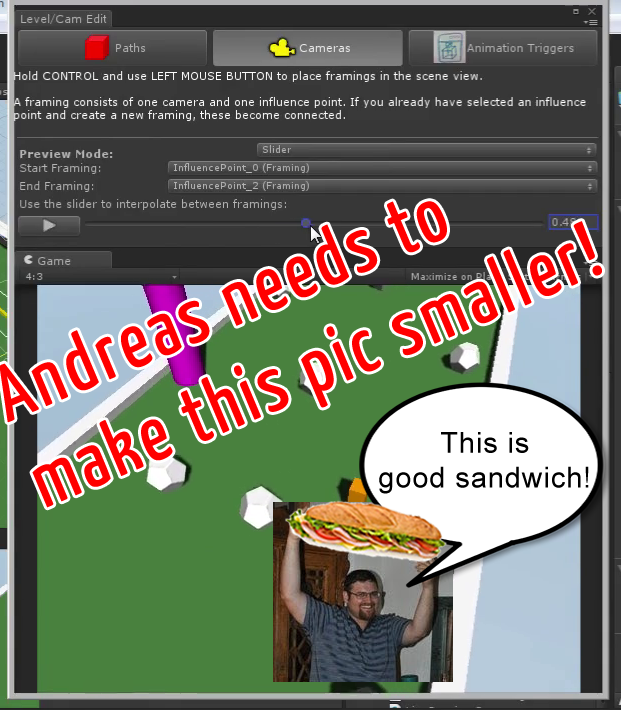
\includegraphics[width=0.45\textwidth]{Pics/slider}
\caption{The slider provides a quick way to preview the framings.}
\label{fig:slider}
\end{figure}

%\subsection{Participatory Design Conclusion}
%It's important to design and iterate with the users' current workflow and mental models in mind. By building on top of their pre-exisiting skills and knowledge, one can ease the learning curve by creating a design that is close to what the users are already familiar with. The users should become co-creators, but you should not forget that \textit{you} are the designer. You should listen to what the users say they want, but even more so try to understand what they really \textit{need} and \textit{why} they need it.
\subsection{Interpolation Between Framings} \label{interpolationChapter}
Each influence point is placed on the player path. The interpolated camera settings ($f_{i}$) are a function of the player's position $P_{pos}$, which is used to interpolate between the camera settings $c_1$, $c_2$ of the two influence points on the path closest to the player's position, with a weights $w_1$ and $w_2$ based on the positions of the influence points.
\begin{equation}
f_{i} = f(P_{pos}) = w_1c_1+w_2c_2
\end{equation}
The two closest influence points are found by a linear search from the player's position along the path segments in both directions. The distance travelled in both directions until encountering an influence point is logged $i1_{dist}, i2_{dist}$.
\begin{equation}
w_1 = {d_1}/(d_1 + d_2)
\end{equation}

\begin{equation}
w_2 = {d_2}/(d_1 + d_2)
\end{equation}
In the case there is no influence point in one direction, the distance in that direction is zero. The artist is further able to manipulate the weights, $w_1$ and $w_2$, for each camera setting through the graph editor. Evaluating the curve at $w$ produces a new weight, $w_{i}$, for each camera settings.

%In pseudo code, this gives us the following interpolation for each camera setting:
%\begin{equation}
%f_{i} = i1_{cam_{i}} * w_{i} + i2_{cam_{i}} * (1-w_{i})
%\end{equation}

\subsubsection{Path-Based Slider-Preview}
For the slider preview, a player position, $P_{pos}$, is computed from the given slider value, $w_s$, from 0 to 1, and the influence points of the start and end framing ($i_{start}, i_{end}$).


\begin{equation}
P_{pos} = f(w_s, i_{start}, i_{end})
\end{equation}


Drawing from the same logic as in the interpolation, a linear search is performed from the influence point of the start framing $i_{start}$ following the path in both directions, logging the total distance travelled until the influence point of the end framing $i_{end}$ is encountered. Using the total distance between the start and end framing, the interval [0,1] is mapped to the sequence of the encountered influence points between the start and end framing. For slider values between two influence points, the position $P_pos$ is computed using linear interpolation.


%Each time the search passes another influence point, it logs it $i_{n}$ together with the distance travelled $i_{n_{dist}}$. All distances $i_{n_{dist}}$ are normalized $i_{n_{distNorm}}$, with the total distance travelled $TD$ set to 1. The slider-weight $sw$ now fits in an interval between two influence point distances $i_{before_{distNorm}}, i_{after_{distNorm}}$). The possible player character position $P_{pos}$ is then calculated and used as the argument in $f_{i} = f(P_{pos})$.
%\begin{eqnarray}
%P_{pos} &=& i_{after_{pos}}\left(1 - \left(sw - i_{before_{distNorm}}\right)\right)\nonumber \\
%&&\mbox{}+ i_{before_{pos}}\left(sw - i_{before_{distNorm}}\right)
%\end{eqnarray}
%where $i_{n_{pos}}$ is the world position of $n$ influence point.
\section{Evaluation}
%Give artists the task to make a video in a certain scene using some specific features, both in Unity and in Maya. We can then compare their performances, and if the two performances are significantly close, the tool was a success.

%Video and audio recordings. Time spent on tasks. Few questions about usability and experience.

%(Hypotheses - not sure yet?)

To evaluate the usage of FCT, we have chosen to focus on testing whether or not the tool allows the artists to successfully perform the tasks that the tool was originally designed for, as mentioned in Section \ref{PD_Findings}.

%To evaluate the usability of the FCT, we conducted a study at The Animation Workshop. The goal was to observe if the FCT allowed the artists from the participatory design group to use the tool both effectively and creatively. Furthermore, to offer a wider perspective, we used a control group without any prior experience with the FCT. This was done to investigate the applicability of the tool with artists that had no prior experience with working with neither games nor the camera tool.

%\begin{enumerate} [noitemsep]
%\item To find out if the FEELS tea's mental models of the camera system match how the system actually works.
%\item Compare other artists from TAW 3rd year using the camera system with the FEELS team.
%\end{enumerate}

\subsection{Method} \label{method}

\subsubsection{Participants}
Two groups of test participants took part in the evaluation: three artists from the participatory design group and three artists outside the participatory design group. Both groups were students from The Animation Workshop. Since the first group was involved in designing the FCT, they had previous knowledge of the tool. The three other artists who knew nothing about the FCT were used as a control group to avoid this bias.
\subsubsection{Procedure}
Each participant was tested individually in a small meeting room (see Figure \ref{fig:test_setup}). Besides the participant, a facilitator and an observer was also present in the room. The test was split into seven parts:

\begin{enumerate}[noitemsep,nolistsep]
\item Consent form
\item Demographic and Introduction
\item Basic Navigation
\item Training
\item Tasks
\item Creative
\item Post-test Questionnaire
\end{enumerate} 

\subsubsection{Demographic and Introduction}
The participant were given a brief introduction and was subsequently presented with a consent form to allow video recording. The participants started by answering a demographic questionnaire on a laptop. After this they were introduced to a demo of the Camera Path Animator (see Section \ref{relatedWork}). They were told to move the player character by using WASD and then notice how the camera behaved accordingly. This was to give the participant context for the test and to introduce them to the concept of camera behaviour in an interactive environment. 

\begin{figure}[htbp]
\centering
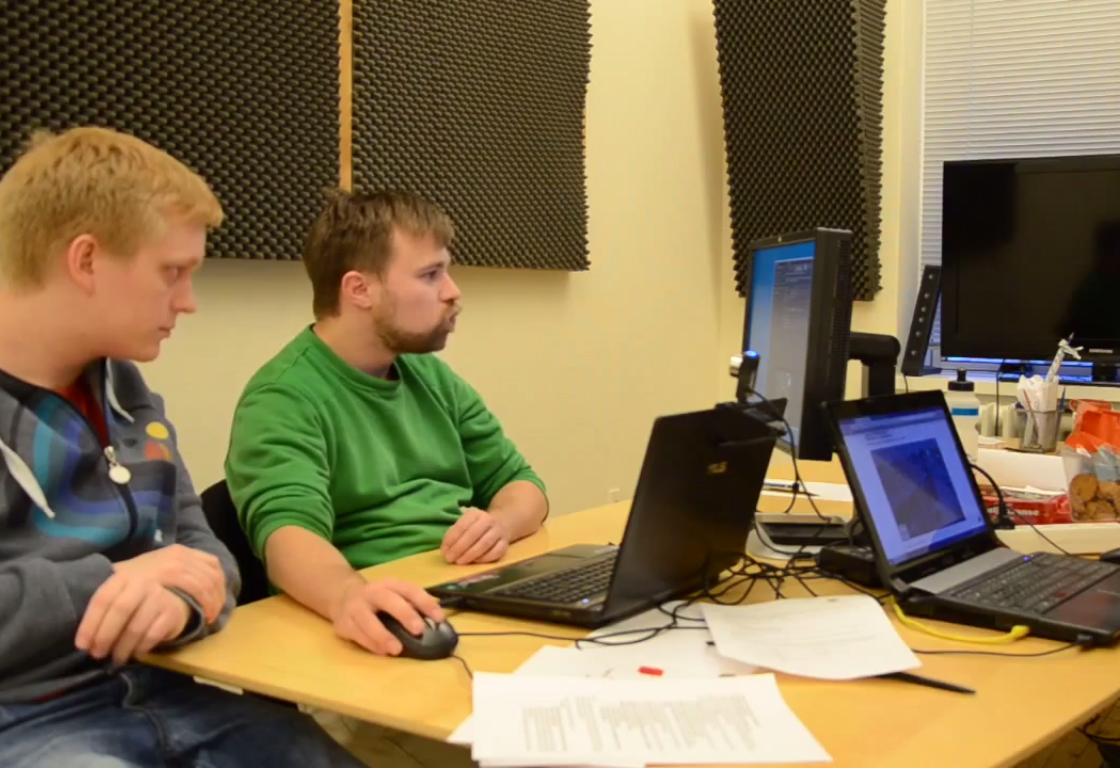
\includegraphics[width=0.3\textwidth]{Pics/test_setup}
\caption{The test participant used had two monitors at his disposal while working with the tool.}
\label{fig:framingConcept}
\end{figure}

\subsubsection{Basic Navigation}
The participants and facilitator sat down at another laptop with a second monitor connected. Here the facilitator gave the participant a basic introduction to Unity so that all participants had no problem understanding the Unity workspace layout, moving around with the scene view camera, changing the position and rotation of objects, etc. To ensure this, the participants was told to move the scene view camera to three positions in the scene (e.g. move camera above the green cube in Figure \ref{fig:sceneAll}). The participant was tasked to move the camera to three specific locations in the environment to ensure they felt comfortable in the workspace. 

\subsubsection{Training} 
After this the facilitator introduced the camera tool to the participant, first he explained the concept using a printed out version of Figure \ref{fig:framingConceptNew}, then he opened the tool in Unity and explained its features and functionalities. The participant tried each feature as they were introduced, e.g. when the facilitator explained how to place influence points and how to connect them, the participant was asked to try it for themselves. 

\subsubsection{Tasks}
When all features were explained, the participant was handed a piece of paper with five tasks. The tasks are as follows:

\begin{enumerate}[noitemsep,nolistsep]
\item Make the camera's field of view change.
\item Make the camera tilt upwards.
\item Make the camera look at the tall pink cylinder.
\item Make the camera go from a low perspective to bird’s-eye view.
\item Change the interpolation of one of the previous assignments by changing the animation curve.
\end{enumerate} 

The chosen tasks reflects five common features and tasks that's often used when setting up a framing and a camera interpolation. The participant had to solve the tasks themselves, the facilitator only intervened when the participant was struggling with something, asked a question, or at unforeseen occurrences (e.g. bugs). 

\subsubsection{Creative}
After this, the participant was introduced to a level with a modelled environment. They were then tasked to envision and sketch two ways for the camera to move as the play character moved through this environment, when they had two ideas, they were tasked to implement both of these using our camera tool. The facilitator remained as neutral as possible for this part of the test, but still intervened if they participant was struggling or encountered things like bugs.

\subsubsection{Post-test Questionnaire}
Finally, the participant went back to the first laptop and answered a post-test questionnaire. The participant was thanked and the test ended.
\subsubsection{Materials}
Three scenes was constructed for the test. The first was an environment with simple geometry scene. The second was used in the first part of the test when participants were introduced to the camera tool and had to complete 5 tasks. The third level was for the creative part of the test when participants had to envision the camera movement in an environment and then implement it. 

\begin{figure*}[htbp]
\centering
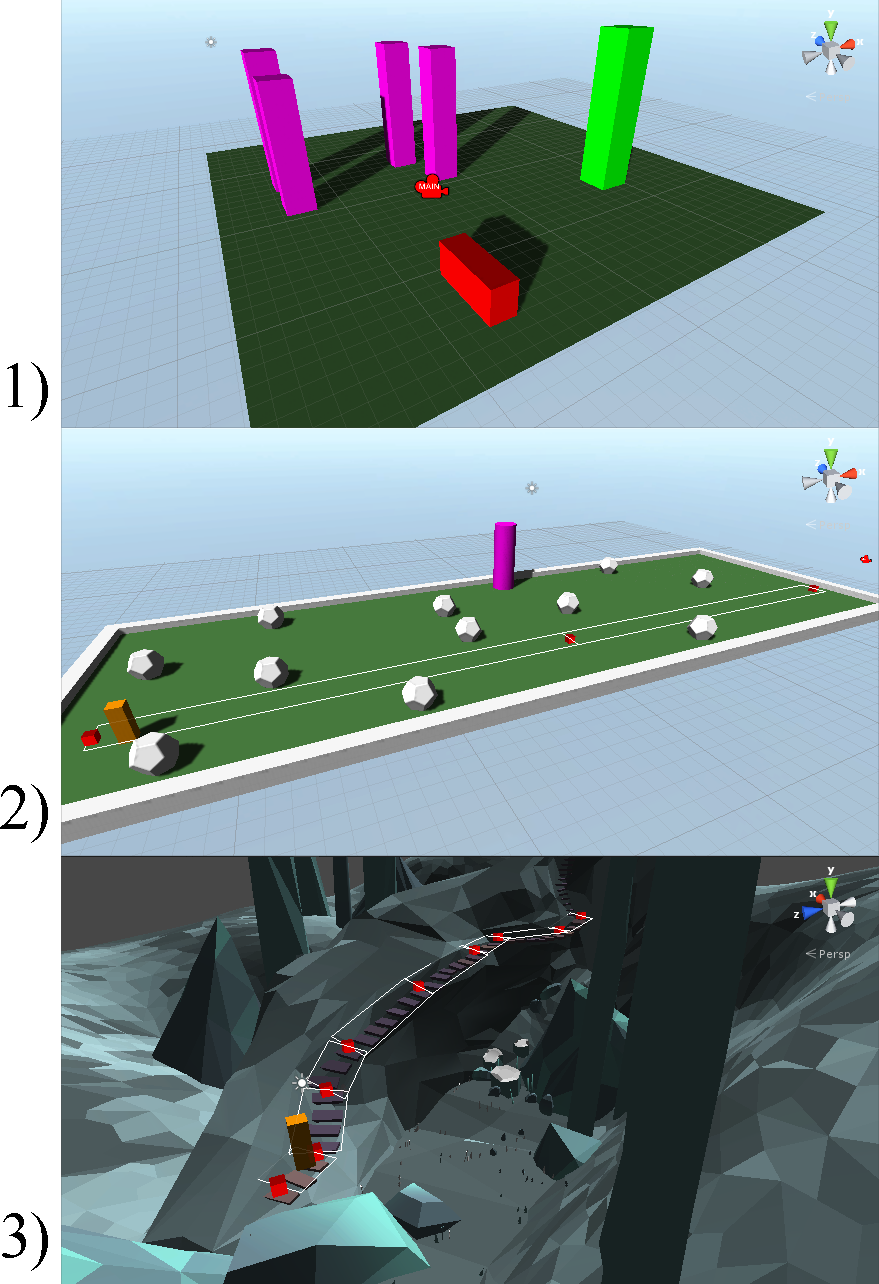
\includegraphics[width=0.45\textwidth]{Pics/sceneAll}
\caption{1) The participant was instructed to move the camera to the top of the green cube, between the purple pillars and to the bottom of the red cube and then rotate the camera to look at the purple pillars. 2) A flat plane with simple geometry to make it easier to see differences when changing camera settings. 3) A mountainous environment with a staircase attached to the mountainside.}
\label{fig:sceneAll}
\end{figure*}
\subsection{Evaluation Questionnaire}
The participants had varied experience with Autodesk Maya, ranging from six months to six years. In Unity, their experience ranged from none at all to more than a year.

The participants rated their agreement with a list of statements using a 5-point Likert scale ranging from ``strongly disagree" to ``strongly agree". 

%While the test participants tried the FCT, they were recorded  their two monitors were. Additionally, a webcam recorded the face of the participants, together with the audio. An observer wrote notes during the evaluation. For the questionnaire, the participants rated themselves on the following statements using a 5-point Likert scale ranging from "strongly disagree" to "strongly agree". 
%\begin{itemize}[noitemsep,nolistsep]
%\item \textit{I felt empowered using this tool.}
%\item \textit{I felt restricted using this tool.}
%\item \textit{I felt I got the tasks done quickly.}
%\item \textit{I felt the tool allowed me to complete the tasks well.}
%\end{itemize}

When asked if the participants \textit{``felt empowered using the tool"}, four participants \textit{agreed}, while the remaining two \textit{strongly agreed}. When asked if they \textit{``felt restricted using the tool"}, five participants \textit{disagreed} while the remaining participant \textit{strongly disagreed}. When asked they if they felt that they \textit{``got the tasks done quickly"}, four participants \textit{agreed} and two \textit{strongly agreed}. To find out how effective the participants felt using our tool, we asked them if they \textit{``felt the tool allowed them to complete the tasks well"}, three participants \textit{agreed} and three \textit{strongly agreed}.

%To find out how efficient the participants felt using the FCT, we asked them if they felt they \textit{"got the tasks done quickly"}. Four participants \textit{agreed} and two \textit{strongly agreed}. To find out how effective the participants felt using our tool, we asked them if they \textit{"felt the tool allowed them to complete the tasks well"}. Three participants \textit{agreed} and three \textit{strongly agreed}.

Furthermore, they were asked whether they preferred the \textit{be the camera} or the \textit{snapshot} feature for adjusting cameras. Four chose \textit{ be the camera} and two chose \textit{snapshot}. 
They were also asked how useful they thought the preview features were. The response choices were ``not useful", ``somewhat useful", ``very useful", ``didn't use any of them", and ``don't know". Five participants found them \textit{very useful}, and one found it \textit{somewhat useful}.
Finally, the participants were asked what their overall favorite feature was. Three participants noted the \textit{be the camera} feature as their overall favourite feature, while the \textit{slider preview} was the favourite for the other three participants. 

To see the full demographic and evaluation questionnaire, see the attached worksheets.

%When asked about the preview features, five participants found them \textit{very useful}, and one found it \textit{somewhat useful}. The participants were also asked whether they preferred the \textit{be the camera} or the \textit{snapshot} feature. Four named\textit{ be the camera} and two named \textit{snapshot}. Furthermore, three participants noted the \textit{be the camera} feature as their overall favourite feature, while the \textit{slider preview} was the favourite for the other three participants. 

%Furthermore, they were asked whether they preferred the \textit{be the camera} or the \textit{snapshot} feature for adjusting cameras. They were also asked how useful they thought the preview features were. The response choices were "not useful", "somewhat useful", "very useful", "didn't use any of them", and "don't know". To highlight the best features in the tool, the participants were asked to name their favourite feature from a list of 7.

%When asked about the preview features, five participants found them \textit{very useful}, and one found it \textit{somewhat useful}. The participants were also asked whether they preferred the \textit{be the camera} or the \textit{snapshot} feature. Four named\textit{ be the camera} and two named \textit{snapshot}. Furthermore, three participants noted the \textit{be the camera} feature as their overall favourite feature, while the \textit{slider preview} was the favourite for the other three participants. 
%\subsubsection{Data Analysis}
The video recordings from the experiment was coded internally at a later date in pairs of two. The two pairs coded one participant in unison and then split up and worked in parallel. Repeated ideas, events and observations was tagged with certain tags. The tags used are \textit{confusion}, \textit{exploration}, and \textit{problem}.

An event was tagged with \textit{confusion} if a participant was confused that a feature didn't work as they expected or struggled doing what they wanted/envisioned (e.g. did not connect influence points; unsure why interpolation didn't not function properly), 
\textit{exploration} means that a participant explored the interface or features of the camera tool by themselves without prompting them or if they asked questions about the features (e.g. \textit{"What consequence does it have if the points are not connected? Would that be a cut?"}), 
%\textit{observation} is an (subjective) observation made internally about the participant and their behavior or approach to the tasks (e.g. no problem navigating in Unity), 
\textit{problem} means a participant got stuck or encountered a problem so they could not progress (e.g. tried changing position of camera while Aim Point was active. The camera jumped around seemingly random in the scene and moved to an unwanted position because of it.)
%\subsection{Results} \label{results}
Four participants reported to have between one and three years of experience with Autodesk Maya, another had between four and six years of experience and the last had seven or more years of experience. Only one participant had more than one year of experience with Unity, another had between six and twelve months of experience with it, the rest reported to have less than six months of experience.
When asked if they \textit{'felt empowered using the tool'}, 2/6 participants \textit{strongly agreed} and 4/6 participants \textit{agreed}.

Coded data shows...



When asked if the participants felt empowered using the tool, four participants agreed while the remaining two strongly agreed. When asked if the they felt restricted when using the tool, five participants disagreed while the remaining participant strongly disagreed. To find out how efficient the participants felt using our tool, we asked them if they felt they got the tasks done quick, four participants agreed and two strongly agreed. To find out how effective the participants felt using our tool, we asked them if they felt the tool allowed them to complete the tasks well, three participants agreed and three strongly agreed.
When asked about the preview features, five participants found them very useful, and one found it somewhat useful. For the participants' favorite feature for adjusting camera positions, four named 'Be the camera' and two named 'Snapshot' as their favorite. Furthermore, three participants noted the 'Be the camera' feature as their overall favorite while the 'Slider Preview' was the favorite for the other three participants. 
%\subsection{Observations}
Quotes, etc...
\section{Discussion}
\subsection{Principles and Guidelines}
General findings that can be learned from this study. Could be something like the "180 degree rule" of games. Examples: that the barycentric interpolation works better than triangulation; that you should at maximum have four cameras; that cutting between multiple cameras confuses the player if the cutting speed is less than X, etc. In short, something the reader can use after having read the paper.
\section{Acknowledgements}
We would like to thank the artists that helped designing the Framing-based Camera Tool. We would also like to thank Anja Perl and Emil Kj\ae hr from The Animation Workshop in Viborg for making this collaboration possible.



%%% old stuff
%\section{Background Knowledge}

\subsection{Eye movements}
To understand how speed reading is possible, it's important to understand some basics on how the eye moves.

When you read, visually analyse or look for something, your eyes are doing a series of movements called \textit{saccades}. In between these movements your eyes shortly fixate on elements, these stops called \textit{fixations}. Each fixations lasts only around 200-300 ms, so our eyes are quickly looking around a scene to find new details to fixate on. Luckily the movements of the eyes themselves are incredibly fast, reaching speeds of 500 degrees a second \cite{MATHIAS KILDE}.


But this all depends on what you're using your eyes for. There is generally three types of saccades: pursuit, vergence and vestibular. \textit{Pursuit} is when your eyes are trying to fixate on something moving. Generally, in these cases, the saccades are slower, as your eyes are following the target and not going back and forth between different targets \cite{KILDE MATHIAS}.
\textit{Vergence} is the inwards movement of your eyes to focus on something getting closer to you \cite{KILDE MATHIAS}.

\textit{Vestibular} movement is the eyes rotating to compensate for body and/or head movement. This is both caused by visual stimulation, but mostly by the vestibular organ in your ears. This is also also why your sight gets blurry when you're dizzy.

In the case of reading, it's also important to talk about the different kinds of small saccades the eyes are capable of. \textit{Nystagmus} is very tiny and quick movements in the eyes, which causes a kind of tremor in your vision \cite{KILDE MATHIAS}. You will notice it when staring intently at a fixed point. It's believed that this is a precaution in the eyes to make the nerve cells keep firing by continuously stimulating them. Furthermore, the eyes also experience small \textit{drifts}. These are believed to be the results of a less-than-perfect control of the oculomotor resulting in your eyes slowly drifting to one side. To accommodate this the eyes make tiny saccades, called \textit{microsaccades}, to realign themselves \cite{KILDE MATHIAS}.

Further, it's important to the understanding of reading is \textit{saccade latency}. Every time a saccade is made, some calculations are needed to approximate where to move the eyes to fixate on a desired target. Even if excluding the uncertainty of where to move the eyes, it would still take 150-175 ms for the initial "request" of moving the eyes to the actual start of the movement. Cognitive processes further increases this latency, but also increases accuracy, meaning your fixation falls closer to the point of interest.
\textbf{
(Gustav: maybe write something about cognitive processes from Perception book here)}

During the saccade, though, everything is a blur. Or it should be anyway. It seems certain parts associated with processing visual inputs are halted during saccades. This process is called \textit{saccadic suppression}. But this is independent of the lexical processing, which means a reader is able to process read text in parallel with saccades \cite{KILDE MATHIAS}.

A fixation is not needed to read a word though. Your attention can be shifted to objects or words in your peripheral vision. But it is not possible to make a saccade without shifting attention to the fixation.

\subsection{Optimal Recognition Position} \label{ORP}
The destination of each saccade when reading, or the fixation point, depends on the content of the sentence; sometimes, the eye also skip words by saccading past them. 80\% of the fixation points are on content words (nouns, verbs and adjectives) and the remaining 20\% are on articles, pronouns, and conjunctions \cite{eysenck_cognitive_2010}. The fixation point inside the words themselves, the \textit{optimal recognition position} (ORP), has an impact on how fast a reader can name the word they are looking at. Research has shown that the ORP is near the middle or slightly left of the middle \cite{oregan_optimal_1992, nazir_letter_1998, oregan_convenient_1984}. The added recognition time as the fixation point deviates from the ORP is a U-shaped curve, see Figure \ref{fig:ucurve}, with around 20 ms added for each letter of deviation.

\begin{figure}[htbp]
\centering
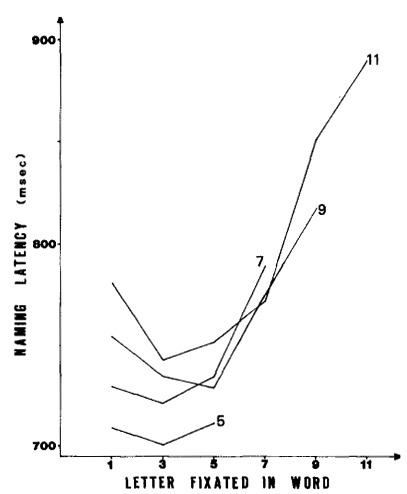
\includegraphics[width=0.4\textwidth]{Pics/ucurve}
\caption{The time it took participants to name the word they saw depending on their fixation point in the word. This graph shows results for words of length 5, 7, 9 and 11. \protect\cite{oregan_convenient_1984}}
\label{fig:ucurve}
\end{figure}

Removing the spacing between words decreases the reading speed with around 30\%. Fixation does not fall on the ORP but tends to the beginning of words. Splitting long words, like long Danish or German compound words, into their individual words, increases reading speed, even though it was grammatically incorrect. Likewise with putting in spaces in Thai, where there are no spaces.

\subsection{Meta-guiding reading (using a pen to keep focus)}
GUSTAV

\subsection{Modes for reading}
BENJAMIN

("gears" - depending on context, you switch "gear"):
Read for memorize
Read for learning
Rauding (sentential integration, lexical + semantic) - most optimal
Skimming (semantic encoding)
Scanning (lexical access? using memory)
Reading rate (WPM) - rauding is the best?
Cognitive speed vs. reading speed
E = AR (E: Efficiency, A: Accuracy, R: Rate)
=======
\subsection{Attention}
MATHIAS

\subsection{Reading Processes}
\citeA{carver_reading_1992} presents five reading processes, also referred to as \textit{gears} (see Figure \ref{fig:trace_cross}). Each gear is defined by its \textit{goal}, \textit{culminating component}, and its \textit{speed}, measured by \textit{WPM} (words per minute). WPM also varies based on reading level, so to block out this bias, \citeauthor{carver_reading_1992} bases his experiments exclusively on college students. The following section is based on his study.

\begin{figure*}[htbp]
\centering
\captionsetup{justification=centering}
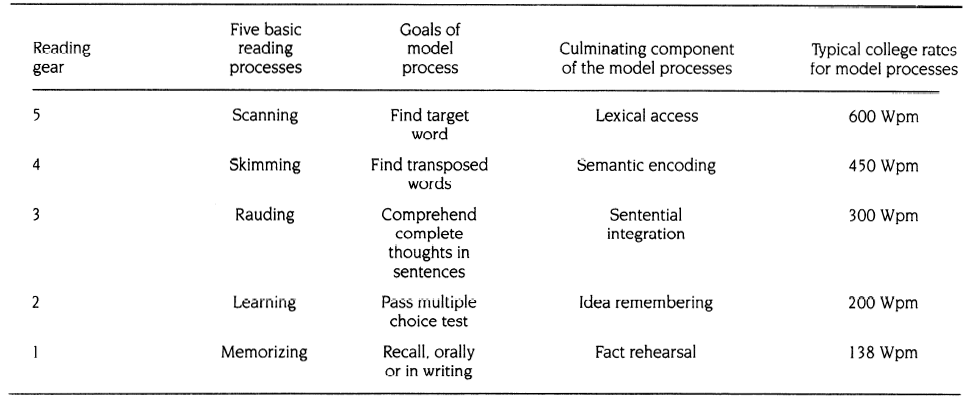
\includegraphics[width=1\textwidth]{Pics/gears_list}
\caption{Each gear has its own goal, culminating component, and WPM. \protect\cite{carver_reading_1992}}
\label{fig:gears_list}
\end{figure*}

The goal relies on the reader's intent when reading the text. For instance, the reader could read the text just to find a single word (scanning). The culminating component of a gear, is then the cognitive process that it requires. \textit{Lexical access} is the component used for finding a single word in memory. If the reader's goal changed to finding a certain sentence in the text, such as in skimming, transposed words must be found and the activity would require an additional component; \textit{semantic encoding}. Other than just finding the words, the reader must now determine the meaning of the sentence. In order for the reader to understand the complete thought of a sentence, the \textit{sentential integration} component must be added. These three components together are the requirement for the most basic and most used reading process - \textit{rauding}, also known as \textit{typical reading}. The word comes from a combination of 'auding' and 'reading', as they both share the same underlying comprehension processes. If the goal of reading the text is to learn, e.g., in order to answer a test, the \textit{idea remembering} component is added. In this gear, some words require re-reading and longer time to process. The final gear is focused around remembering the text and uses the \textit{fact rehearsal} component. This gear requires rehearsing the material and memorizing it. 
\citeA{carver_reading_1992} goes on to mention that the best readers shift up and down in gear while reading, based on the difficulty of the material - a term called \textit{process flexibility}. 

By having college students read a text followed by answering two multiple choice tests, as well as judging their own performance, \citeauthor{carver_reading_1992} tested efficiency at different reading rates. It was found that the students were most efficient at rates around 300 WPM - the rauding reading rate. This rate has therefore been referred to as the most optimal reading rate.
%Efficiency was calculated from the product of accuracy and reading rate, and the accuracy was determined through multiple-choice tests as well as self-judgement.

\citeauthor{carver_reading_1992} also mentions the term \textit{cognitive speed}, which acts as a limit of the reading speed. If the reader passes this limit, he will not be able to operate the culminating components successfully, resulting in a poor comprehension. The main concern however for most students is to make the reading speed reach the limit of the cognitive speed.

\textbf{(Gustav: maybe remove this quote?)}

\citeauthor{carver_reading_1992} describes how the \textit{rauding theory} relates to the \textit{schema theory}. The schema theory uses gears 1 and 2, but mainly focuses on how readers learn or memorize text. \citeA{widmayer_schema_2005} presents schema as a set of rules that help processing new information by interpreting and predicting situations occurring in the environment. Specifically for reading, \citeauthor{widmayer_schema_2005} claims that:

 \emph{''...Correspondingly, teachers of reading have found that activating a learner's schema enables them to better process information that they are reading. Therefore, many advocate teaching learners metacognitive strategies designed to activate one's schema before reading, such as reading heading and the title, looking a visuals in the text, and making predictions based on the title and pictures.''}

This might indicate that when using schema, readers use skimming or scanning before reading a text, but shift to the memorization and learning gears as soon as they start reading. It also indicated that a complete overview of the text can be relevant in some cases.

%(INSERT REF: Reading for One Second, One Minute, or One Year) compares four different theoretical perspectives in reading, each focusing on a certain style and speed of reading: Rauding, Verbal Efficiency, Schema, and Whole Language.

\subsection{Sub-vocalization}
\citeA{bruinsma_should_1980} says that ...
%http://www.jstor.org/stable/20195232
%[Conclusions The evidence cited here should caution teachers to be very careful in their efforts to reduce subvocalization during silent reading. This should be done directly only with students who are otherwise compe tent readers and who are reading relatively easy material ...]

%\section{Preliminary Study}
We did bla bla bla ...

\subsection{Participants}
	Interviews (Knapnok Games, Unity Studios)
	Online questionnaires (27 game developers)
	Observations (4-5 students at TAW)
	
	The interview sessions involved a total of three people from two game studios in Denmark; Project Lead at Knapnok Games in Copenhagen and Lead Designer and Lead Programmer at Unity Studios in Aarhus.
The online questionnaire received 27 submissions from people with a median professional experience of 3 years (SD 2.67).
Lastly, the participatory paper prototyping was done on 4 students at TAW. (from the team?!)

	
\subsection{Methods}
		Interview design (semi-structured)
		Questionnaire design
		Observations (from meetings, discussions)
		Paper prototyping
		Participatory design
		
		The interviews were conducted at the respective companie' offices using a semi-structured approach. The interviews was audio recorded and notes were taken during the interview. We were offered to see the tools they use in production in practice. The session at KnapNok Games took one hour and two hours at Unity Studios.
The questionnaires was published on relevant game development communities. (unity forum, tigsource, 3Dboss.com, game dev facebook groups and twitter). The questions in the questionnaire and the semi-structured interview was designed to be case-specific (hendrik bog) in hope of gathering more detailed information. Both the interviews and questionnaire was analysed with using grounded theory
The paper prototyping was a participatory design - dialogue-based prototyping session. The participants wrote down their requirements while thinking aloud. They then designed their "dream interface" using paper blocks. They expressed their decisions and ideas while doing so. A facilitator would ask why they needed certain elements and why it was chosen to structure it as they did.


\subsection{Findings}
	Frequently mentioned points
	
	The two game studios that were interviewed both use Unity in their development and mentioned that it is most efficient if everyone on the development team is able to use Unity. This allows team members non-programmers (e.g. artists and designers) to implement assets themselves as well as tweak parameters and build functionality using tools made by the programmers. This way, the amount of interactions between programmers and non-programmers are minimized, and non-programmers can take on more tasks.
Among the tools made for non-programmers was 
Points derived from the questionnaire mentions the more tweakable  your design is, the better, i.e. changing variables without going into the code in a text editor. However, this can also be of nuisance as the number of accessible variables can confuse them. A tool also have to be presented clearly. Finally it is important that the designers know the tools they are working with.
During the paper prototyping, the participants continuously mentioned Maya (the software package they're most accustomed to) when trying to explain how they had envisioned the camera tool working; they wanted something close to Maya.

%\section{Participatory Design}
An initial mockup of the tool's interface and functionality was created internally. The mockup had the interface all gathered in one window to keep the design minimalist. However, in search of a better design, we included the end-users in the process going forward (see Figure \ref{fig:mockup}).

To ground our design work, we were interested in learning more about our users and how they envisioned the finished product. Therefore, three participatory exercises were conducted \footnote{The exercises were video documented, except for one artist and half of the footage from another artist in the first exercise}. The first of which was done to know their general workflow when working with cameras in the tools they, namely Maya and Unity. Secondly, we wanted to know which features they requested and how they envisioned the finished tool. Finally, they tried using a prototype of the camera tool based on their initial design and feature requests.


\begin{figure}[htbp]
\centering
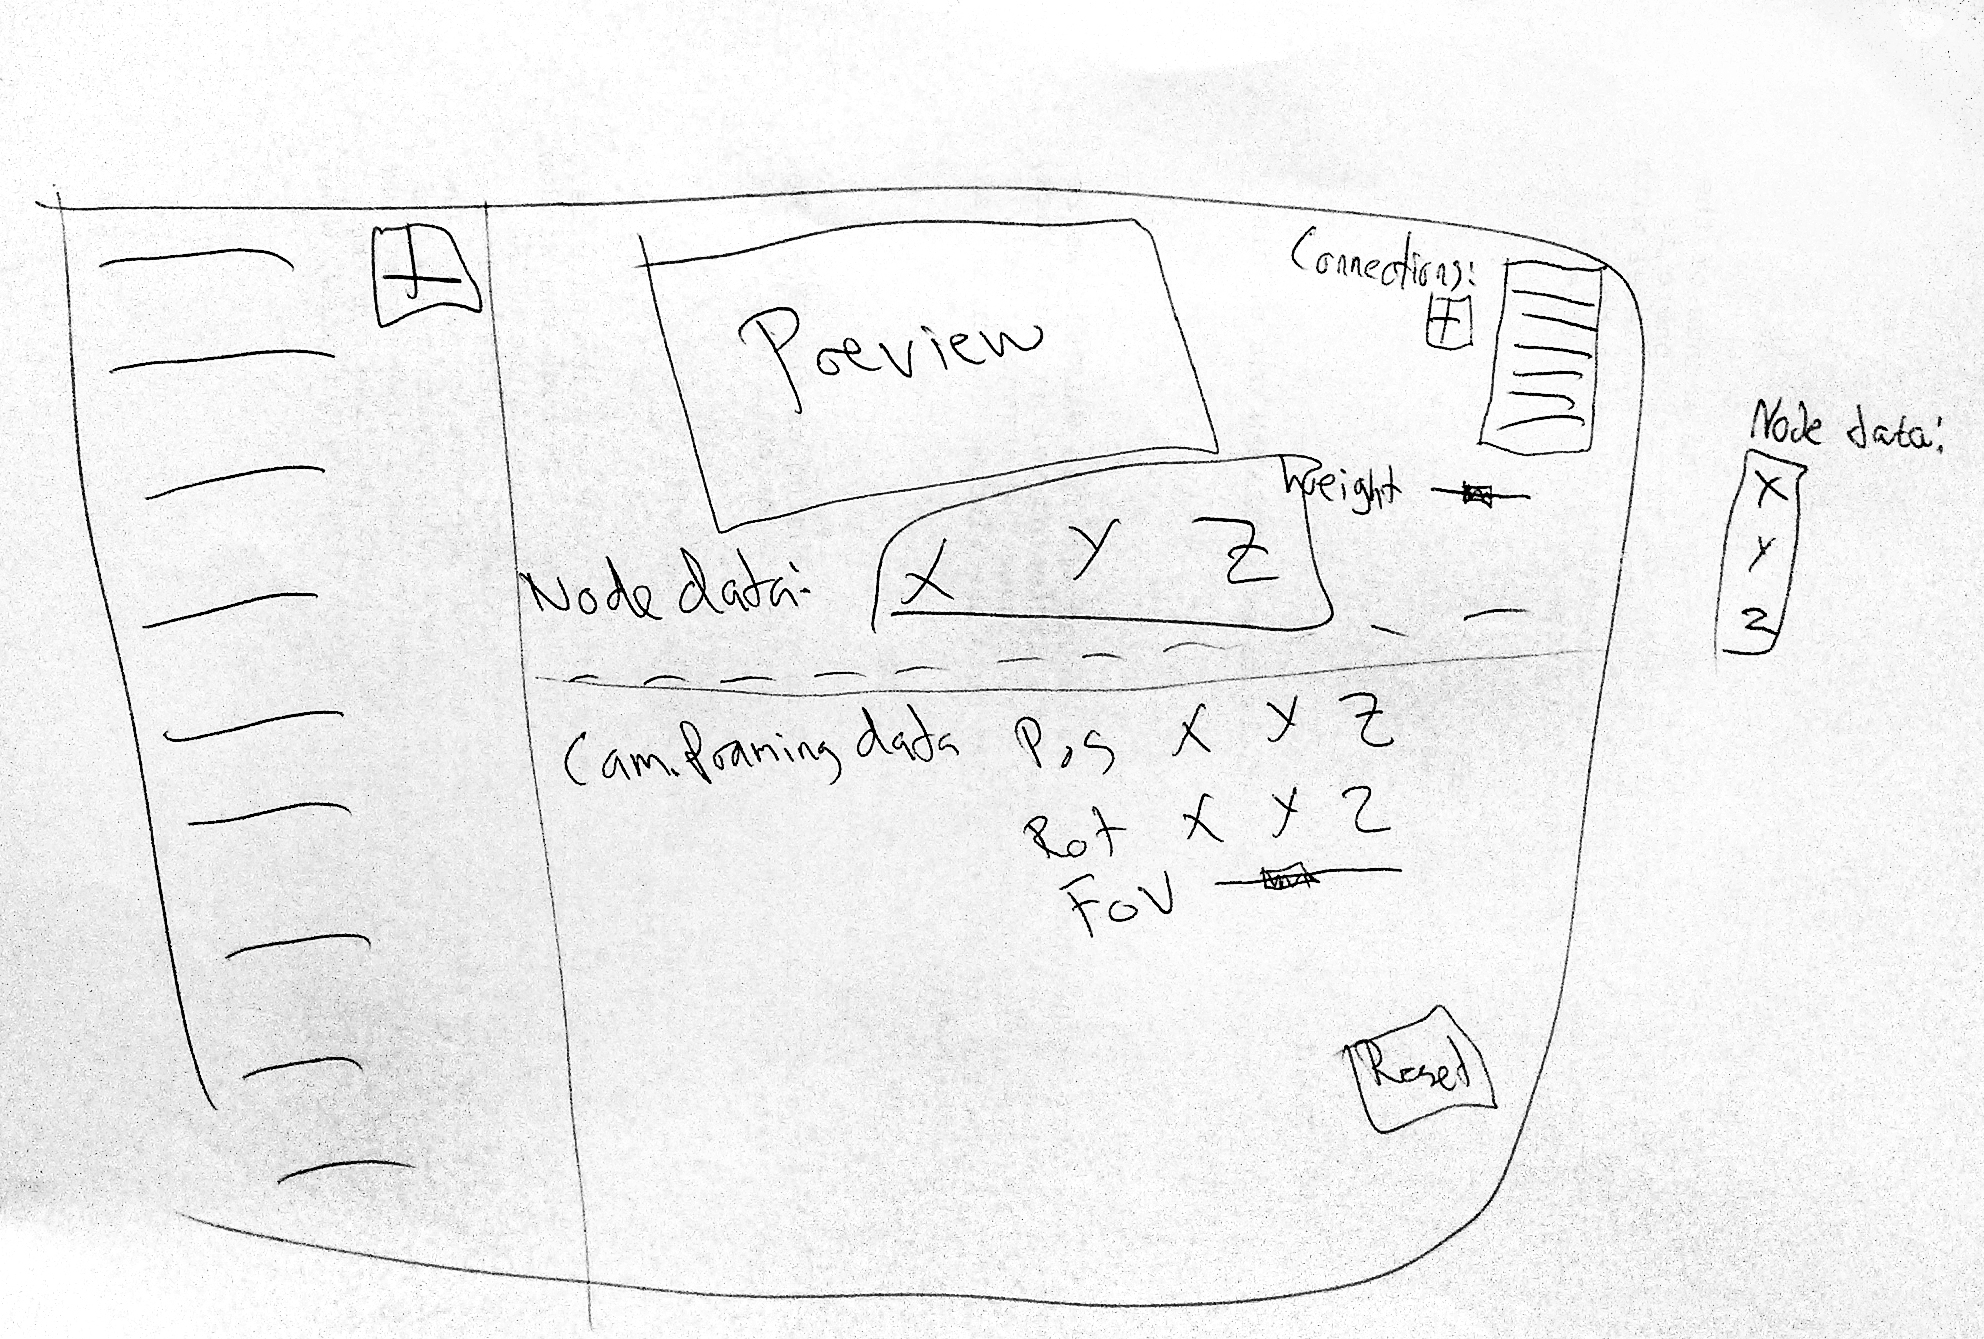
\includegraphics[width=0.50\textwidth]{Pics/InitialMockup}
\caption{The initial concept was to have all the feature tools inside one big window. Early on it was observed that all of the students from The Animation Workshop use a dual-monitor setup, they could then dedicate one monitor to the camera tool.}
\label{fig:mockup}
\end{figure}

\subsection{Exercise 1: Knowledge of tools} \label{exerciseOne}
An artist and a facilitator sat down in front of the artist's work area. The facilitator then asked the artist to show him how he would animate a camera around an object in Maya (see Figure \ref{fig:mads_dual}). This included keyframing and how to change the camera settings for each keyframe. This was done to get an idea of how they usually work. If our camera tool should be successful at helping these artists, it should mimic some of the same behaviour that Maya has. It seemed ideal that the users should be able to utilize their previously-gained knowledge from Maya wherever applicable.

\begin{figure}[htbp]
\centering
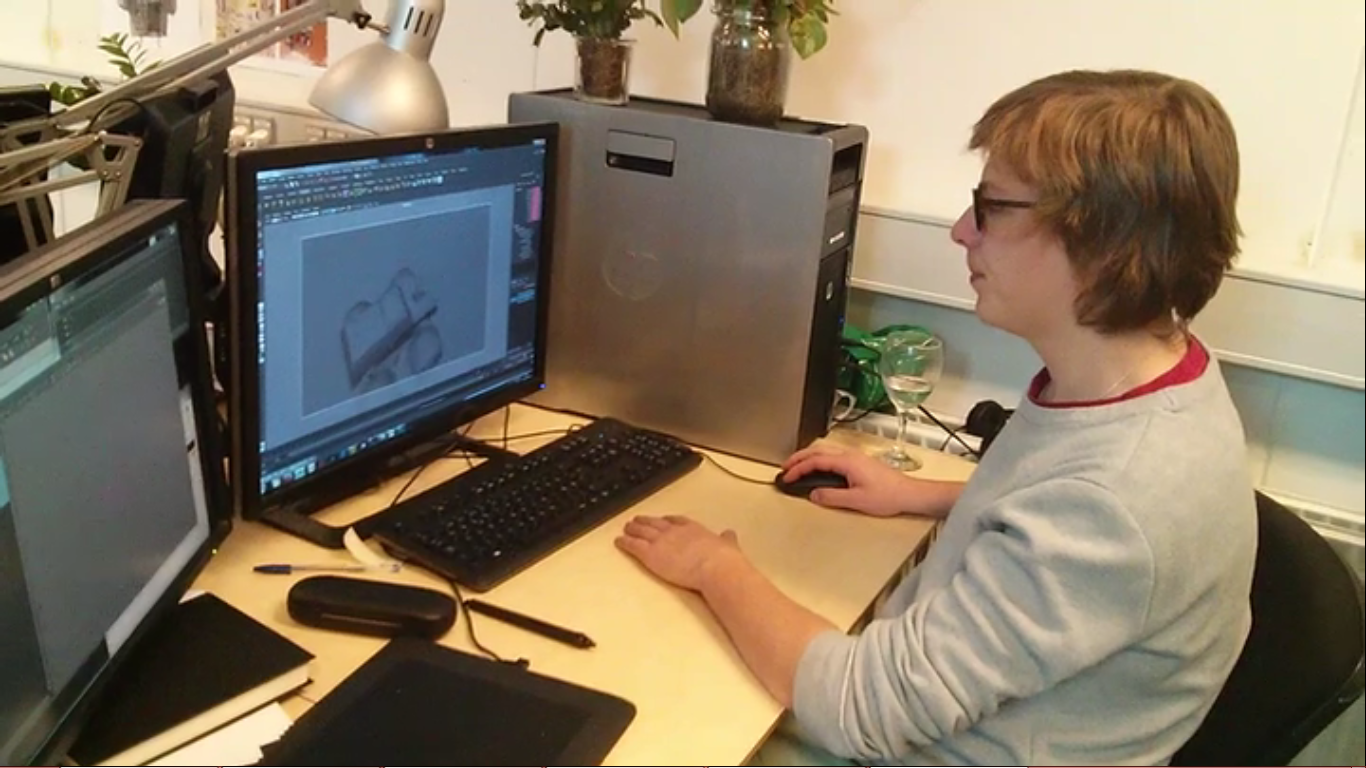
\includegraphics[width=0.50\textwidth]{Pics/Mads_dual}
\caption{All the students at The Animation Workshop work with a dual monitor setup.}
\label{fig:mads_dual}
\end{figure}

After this, the facilitator and artist switched to Unity where he was tasked with moving around in the scene and then to create basic objects such as cubes and spheres, as well as positioning the camera. The purpose of this was to get an understanding of how skilled they are at using Unity - moving around the scene, rotating and translating objects etc. This was done with another two artists as well. The first section of the exercise, the Maya part, was the same for all three artists, but the questions and tasks changed in the last section as the facilitator gained new knowledge about their skill level.

It was discovered that none of the artists knew how to use a standard Unity feature that lets the player fly around with the scene camera as if they were playing a first-person game ("Flythrough Mode", \cite{unity_flyMode}). The artist were excited about the discovery of this feature. One artist perceived the standard way of moving around in Unity as confusing, while another stated that the way of moving the camera is exactly like in Maya. After testing this ourselves, we concluded that the movement controls in Maya and Unity are indeed very similar (except for the "Flythrough Mode"), which means that the artists should ideally be comfortable with navigating in either of the applications.

\subsection{Exercise 2: Feature list and paper prototyping}
The artists were given a blank sheet of paper and a pen and was tasked to draw and write about the camera tool, as they envisioned it in a free-form approach. They then explained what they did and they had a discussion about it. There were no strict requirements of how they approached the task, so some focused a lot on feature requires, while others were more interested in fundamental workflow and user interfaces. This was done with four artists in total.

After this, the same four artists were placed at a desk, one by one, where a variety of labels were laid out in front of them (see Figure \ref{fig:labels}). These labels were marked as different sliders, buttons, windows, field parameters, camera settings, etc. The labels were primarily based on the basic building blocks of Unity's user interface, as well as some of the observations from the first exercise where the users talked about how they worked with Maya.


\begin{figure}[htbp]
\centering
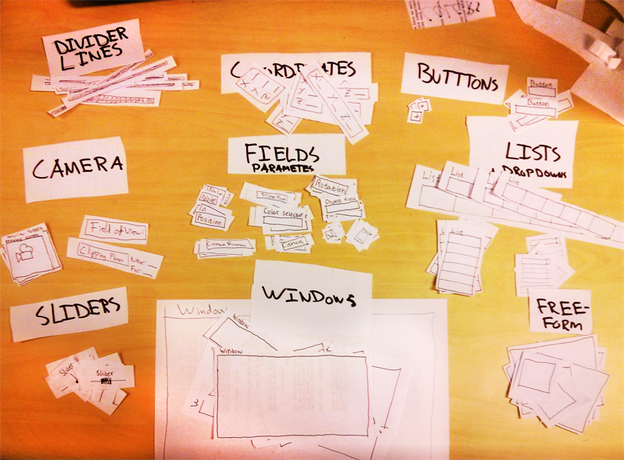
\includegraphics[width=0.50\textwidth]{Pics/labels}
\caption{The users were asked to design their "dream program" by using paper labels as building blocks. They were also allowed to draw their own components if necessary.}
\label{fig:labels}
\end{figure}


All artists wanted basic features like translation, rotation, field of view of the camera, as well as a curve editor to change the interpolation between two cameras. After these features, all the artists diverted in their designs. All the designs were discussed internally and main points and ideas were extracted from them. These findings were used as the foundation of the tool's design. However, the foundation for the program was not strictly based on the artists ideas and requirements; instead, we tried to extract some more general requests of what they as artists actually need. It was important to keep in mind that working in an interactive medium such as game development was a new experience for the users.

A slider that could be used to interpolate between two camera framings in a preview window is an example of an idea that was discarded by us. The artist wanted two preview windows of the camera framing, as well as a preview window of the interpolation, which the slider would manipulate. His idea was similar to a DJ turntable. After discussing it internally, we concluded that this idea would make the interface too elaborate, but the idea of being able to preview your changes quickly was kept.

See Figures \ref{fig:morten_requirements} and \ref{fig:mads_turntable}.

% morten
\begin{figure}[htbp]
\centering
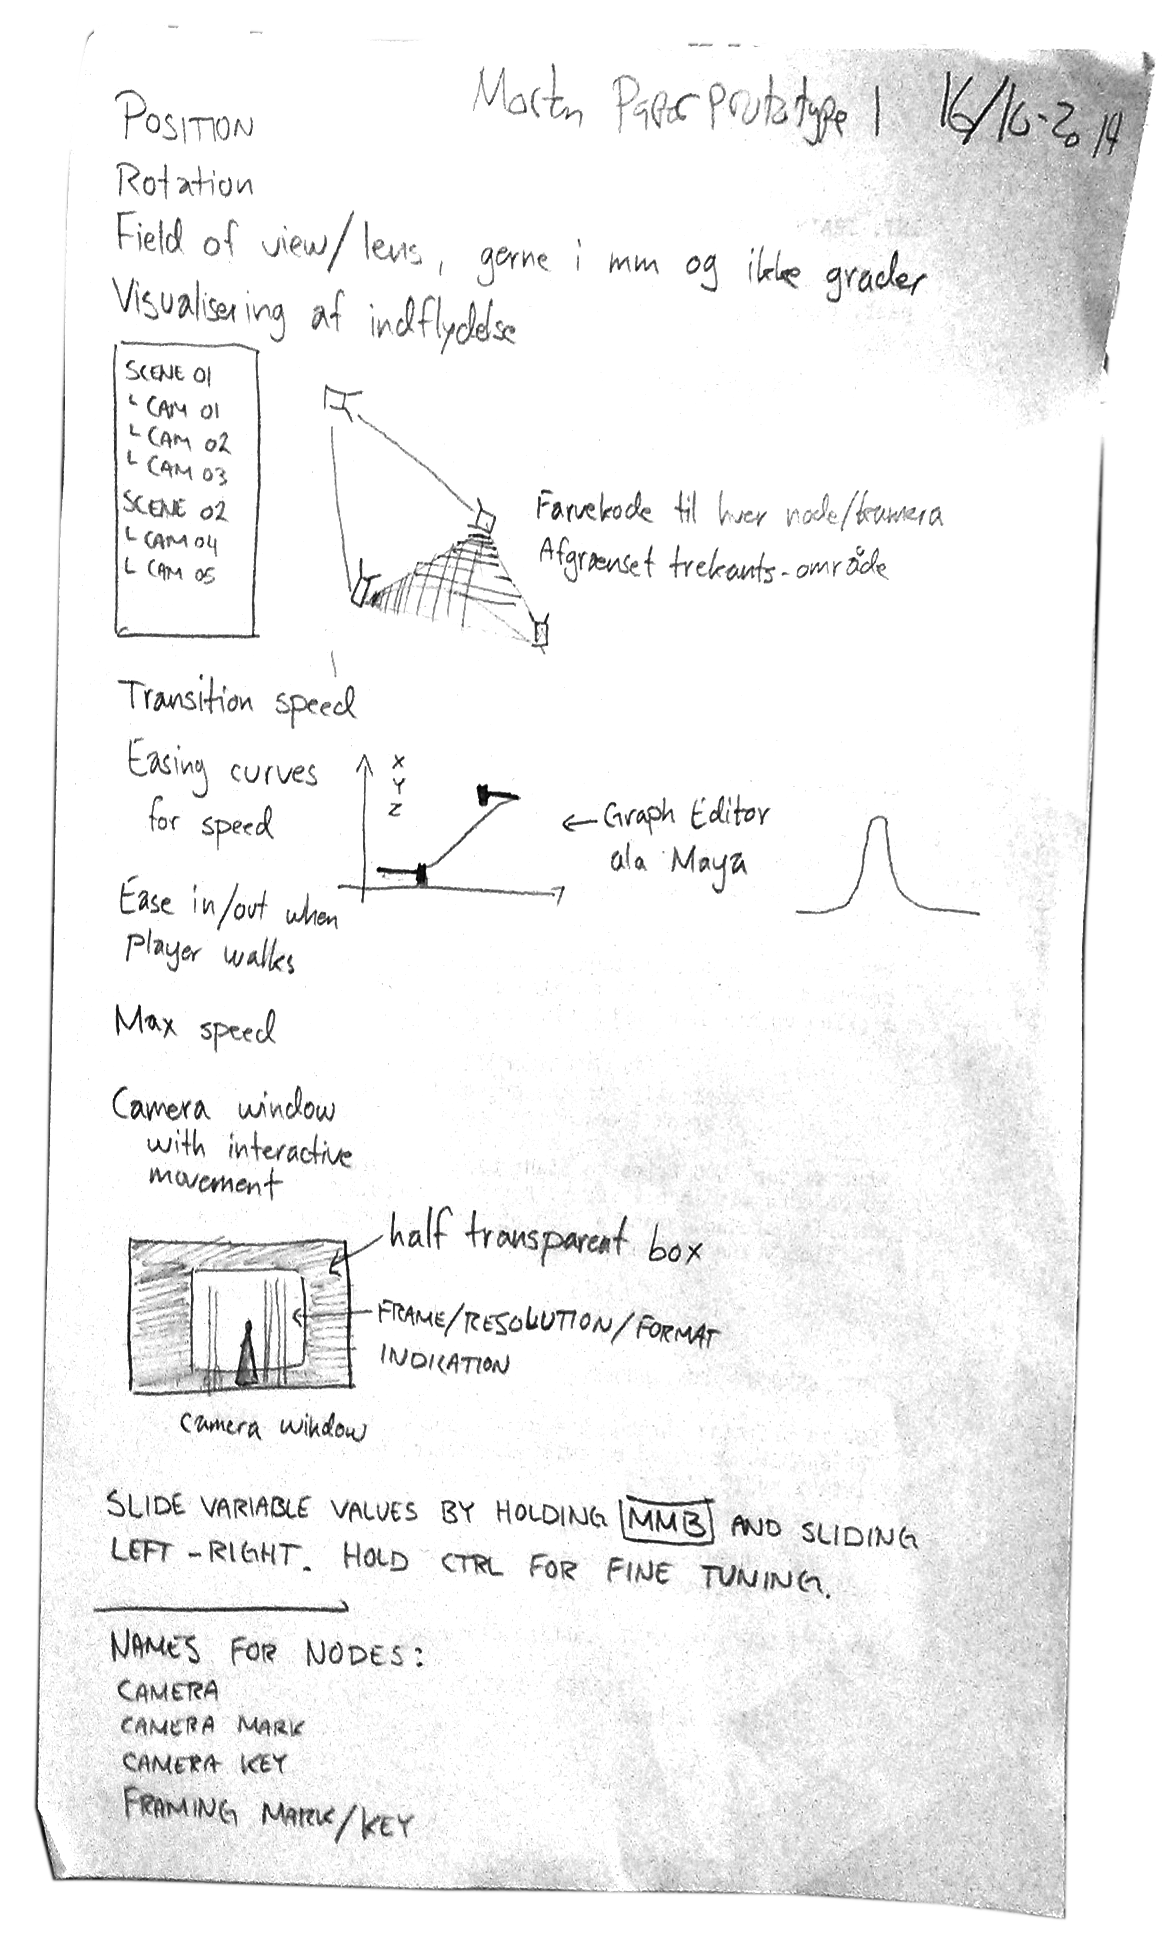
\includegraphics[width=0.50\textwidth]{Pics/Morten01}
\caption{Feature requirements.}
\label{fig:morten_requirements}
\end{figure}

% mads
\begin{figure}[htbp]
\centering
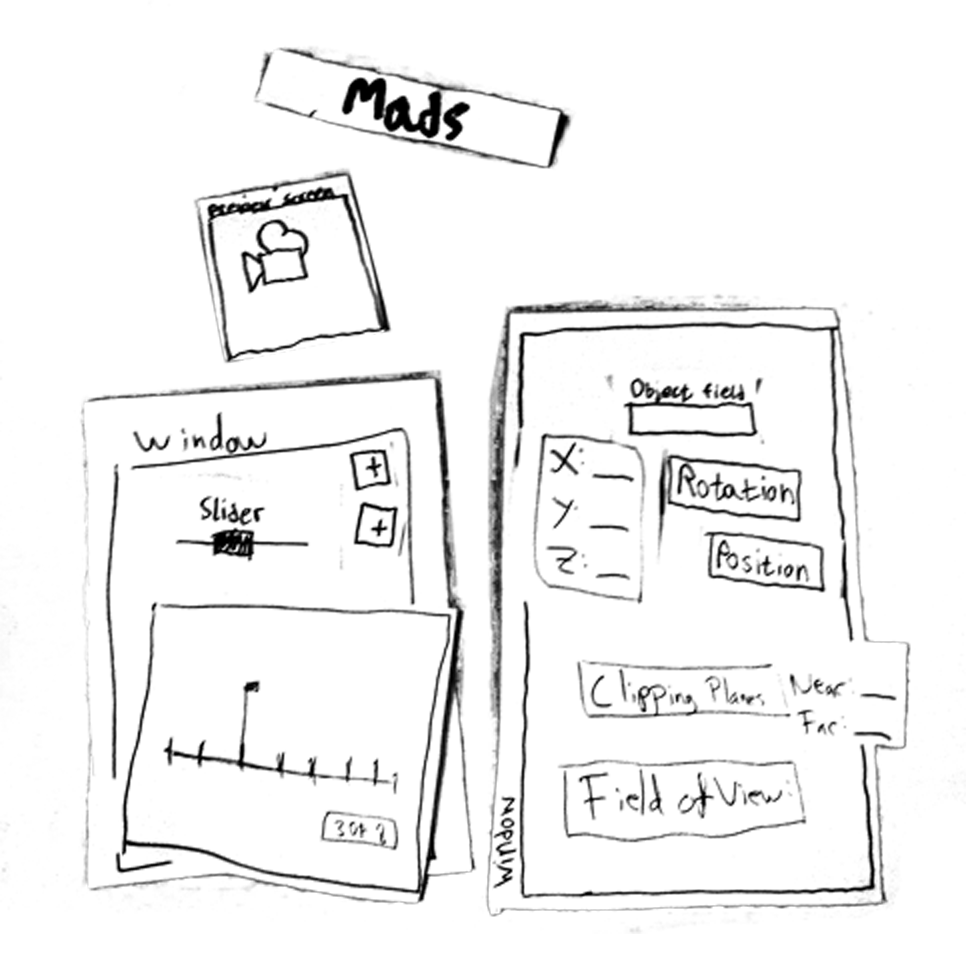
\includegraphics[width=0.50\textwidth]{Pics/Mads01}
\caption{Turntable concept.}
\label{fig:mads_turntable}
\end{figure}

\subsection{Summary of Findings}
\begin{itemize}
\item Basic translation and rotation
\item Field of View
\item Camera modes
\item Domains/areas/trigger zones
\item Toggle camera to either follow or be static
\item Curves and graph editors
\item Quick real-time preview
\item Have triangle in UI that represents the three cameras. Have a 'object' inside that you can manipulate to change the preview (like yellow man in Google Maps)
\item Camera lenses and effects (fish-eye, etc.)
\item Use "aim point" to place the camera
\item "Be the camera" when positioning it
\item Easing (maybe presets?)
\item Hotkey to set new camera mark ("S")
\item Different controls modifiers 
\item Hold shift/ctrl/alt to decrease/increase increment / step size
\item Color code the camera keys/markers
\item Use preview screen as separate window to put on secondary monitor
\item 2D overview of the map with all camera keys/markers
\item When looking through the camera, have transparent border (like in Maya)
\item In camera preview, show what camera is currently 'dominant' (how much weight each camera is pulling)
\item Separate windows that can be docked
\item Allows for multi screen setup
\end{itemize}

\subsection{Exercise 3: First iteration}
After having completed the two exercises, we started developing a rough prototype in Unity (see Figure \ref{fig:prototype}). This iteration included basic functionality to make it possible to test and get feedback as quickly as possible. During one of their daily SCRUM meetings, we presented the tool, as well as providing them a short manual (SEE APPENDIX A).


\begin{figure}[htbp]
\centering
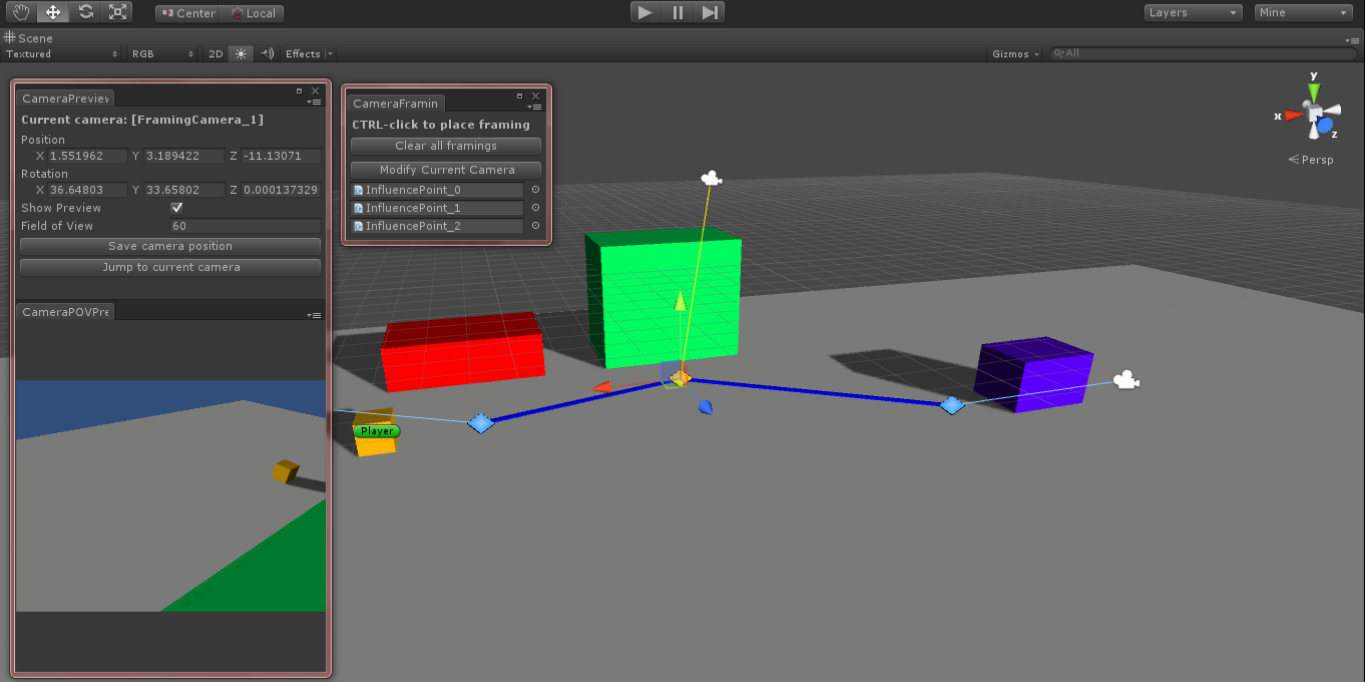
\includegraphics[width=0.50\textwidth]{Pics/MainSetup}
\caption{Rough prototype with basic camera manipulation.}
\label{fig:prototype}
\end{figure}

Three artists tried it out for 10-40 minutes each. They got a chance to try out the tool, as well as expressing their overall opinion about how they preferred the workflow to be.


The facilitator gave the artist small tasks like “Can you place Framings along this paths?” and “Can you try and set the Framing’s camera settings as you’d like?”. This exercise was semi-structured, and not all questions were predetermined; some was thought up as the exercise went on.

Over the course of the exercise, some key points was discovered through observation or discussion with the artist. The biggest piece of feedback revolved how the users are supposed to place the virtual camera in the scene. Initially, users were supposed to use Unity’s "Flythrough Mode" (see Section \ref{exerciseOne}) and place the camera as they liked. Then, they should press the "Save camera position" button (see Figure \ref{fig:prototype}). However, some users were confused about this, since they thought that they now they continuously looked through the camera's point of view, i.e. if they moved around after they'd pressed the button, the framing camera should be changed as well. This was not how the system worked, since it simply just saved the scene camera's position to the framing camera whenever the button was pressed. In other words, the users mental models didn't fit with how the tool worked.
 %% <--- we dont use this anymore
%%%\section{Design Requirements}
 %% <--- Benjamin
%\subsection{Findings}
GUSTAV. They like Maya
\subsubsection{Keyframing Concept}
Through our observations of the artists' use of Maya and from feature request by the artists, we found that the most important feature was keyframes. A keyframe is an event and/or change in one or more parameters over time. Each keyframe corresponds to a point in time, meaning that when the animation reaches this point in time, the values of this keyframe are dominant. Usually this means that in between keyframes some interpolation is happening. This interpolation is per default either linear or uses Bézier curves, but can be manipulated in a graph editor. Anything that can be represented by numbers can be manipulated through keyframes.

But games are dynamic, not linear, so this means keyframes can't be associated with a point in time. Specifically for this game, the camera settings would change according to the player's movement, so keyframes needed to be associated with this. Furthermore, the player had to walk on a fixed path, which made the interpolation significantly simpler.

A quick paper prototype of the initial concept showed promise, and the idea of associating keyframes with player position was easily understood. To avoid confusion, these keyframes were renamed \textit{framings}. A framing consists of an \textit{influence point} and a camera (Andreas' tegning). When the player's position is the same as an influence point, that framing will dominate, meaning the main camera will use the camera settings of the associated camera. Moving between influence points causes an interpolation between each camera setting. This interpolation can be manipulated in a graph editor, as in Maya.

Figure text: The red nodes are indicating the player path, and the yellow nodes are the influence points. %% <--- Gustav + Mathias
%\subsubsection{Adjusting the Camera}
In 3D animation software, there are multiple ways to accomplish the same thing. An example of this is how to position a camera in the scene. This can be done by manually adjusting the X, Y and Z position of the camera; moving it by dragging a handle tool; or, alternatively, by using the the \textit{Look Through Selected} feature \cite{maya_lookThrough}. During the initial observations, it was clear that many of the artists at The Animation Workshop preferred this feature. This concept was translated directly into the camera tool. Using the \textit{be the camera} feature (see Figure \ref{fig:beTheCam}), the artists can place their camera by navigating the scene in Unity with the \textit{Flythrough mode} \cite{unity_flyMode}.

\begin{figure}[htbp]
\centering
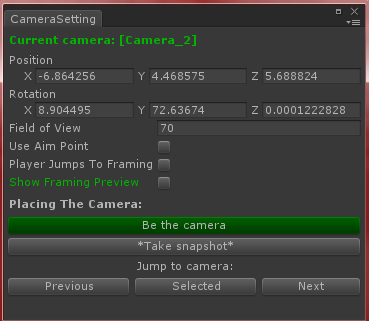
\includegraphics[width=0.3\textwidth]{Pics/be_the_cam_new}
\caption{Pressing the green button puts the user in a special mode where the selected camera inherits position and orientation data from the scene camera. To exit the mode, the user has to press the button again (which now spells "Exit the camera" in red).}
\label{fig:beTheCam}
\end{figure}

Another way to position the camera in Maya is by using an aim-vector control point \cite{maya_camAim}. The artists at The Animation Workshop used this to quickly make the camera aim at something in the scene. This concept has also been designed for the camera tool (see Figure \ref{fig:aimPoint}).

\begin{figure}[htbp]
\centering
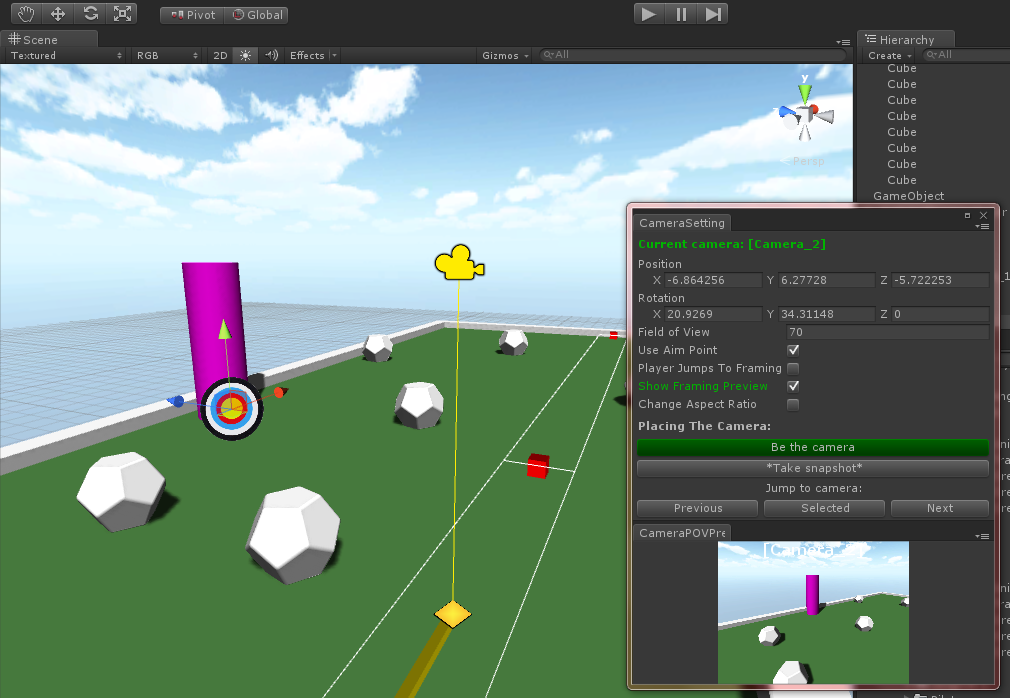
\includegraphics[width=0.3\textwidth]{Pics/aimPoint}
\caption{The aim point allows for quick adjustments of the camera.}
\label{fig:aimPoint}
\end{figure}

%It was discovered that none of the artists knew how to use a standard Unity feature that lets the player fly around with the scene camera as if they were playing a first-person game ("Flythrough Mode", \cite{unity_flyMode}). The artist were excited about the discovery of this feature. One artist perceived the standard way of moving around in Unity as confusing, while another stated that the way of moving the camera is exactly like in Maya. After testing this ourselves, we concluded that the movement controls in Maya and Unity are indeed very similar (except for the "Flythrough Mode"), which means that the artists should ideally be comfortable with navigating in either of the applications.

\subsubsection{Immediate Feedback \& Quick Preview}
An important aspect for the tool was to provide clear feedback. A common request from all of the artists were the ability to quickly preview their changes. Instead of having to start the game and navigate the player character to a specific framing, the artists wanted to quickly jump to a specific framing to test out how it feels and looks.

The artists suggested that they should be able to move the player character around in the editor. Initially, this seemed like a fine way to preview the framings. We considered this option, but deemed it a bit impractical, since it sometimes would be hard to locate the player character in a big scene. Instead, we took inspiration from Camera Path Animator 3.0 mentioned in Section \ref{relatedWork} by designing an interactive slider. With this feature, the artists are able to choose the start and end framing. By dragging the slider between those, the artists can quickly get a feel of how the camera movements will look (see Figure \ref{fig:slider}).

\begin{figure}[htbp]
\centering
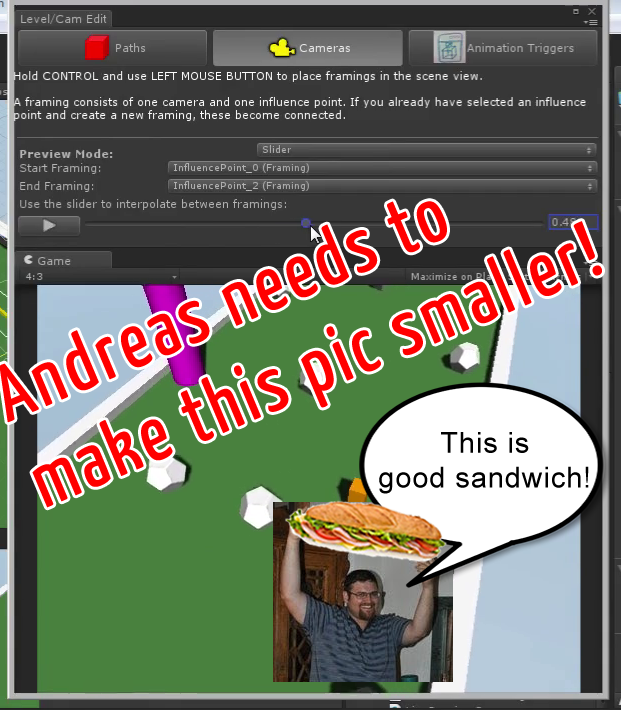
\includegraphics[width=0.3\textwidth]{Pics/slider}
\caption{The slider provides a quick way to preview the framings.}
\label{fig:slider}
\end{figure} %% <-- Gustav
%\subsection{Participatory Design Conclusion}
It's important to design and iterate with the users' current workflow and mental models in mind. By building on top of their pre-exisiting skills and knowledge, one can ease the learning curve by creating a design that is close to what the users are already familiar with. The users should become co-creators, but you should not forget that \textit{you} are the designer. You should listen to what the users say they want, but even more so try to understand what they really \textit{need} and \textit{why} they need it. %% <-- Gustav
%\input{ourapproach}

%%%% ---------- How to make headlines and sections ---------- %%%
\section{This is a section} \label{sec:thisSection}
\subsection{This is a subsection}
Let us refer to section \ref{sec:thisSection}.

%%% How to write bold, italics %%%
This text is \textbf{bold}.
This text is \textit{italics}.

%%% ---------- Insert page break ---------- %%%
%%\newpage
%%Here is some text on the next page

%%% ---------- This is how you refer to a figure in the text ---------- %%%
Here is something that I illustrate in figure \ref{fig:wavelength}.

%%% ---------- This is how you insert a single picture ---------- %%%
\begin{figure}[htbp]
\centering
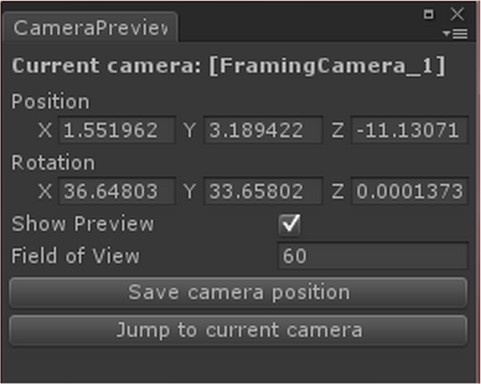
\includegraphics[width=0.50\textwidth]{Pics/Dummy}
\caption{Image caption text goes here bla bla bla bla}
\label{fig:wavelength}
\end{figure}

%%% ---------- This is how you insert multiple pictures ---------- %%%
\begin{figure}[htbp] \centering
\begin{minipage}[b]{0.45\textwidth} \centering
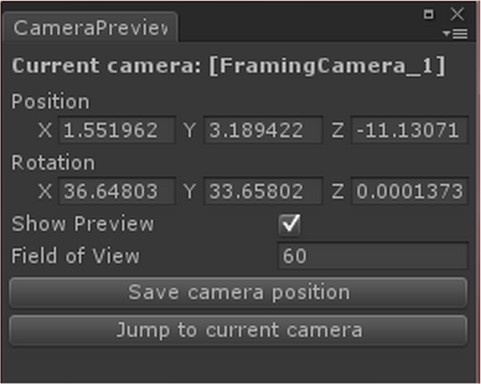
\includegraphics[width=0.60\textwidth]{Pics/Dummy} % Venstre billede
\end{minipage} \hfill
\begin{minipage}[b]{0.45\textwidth} \centering
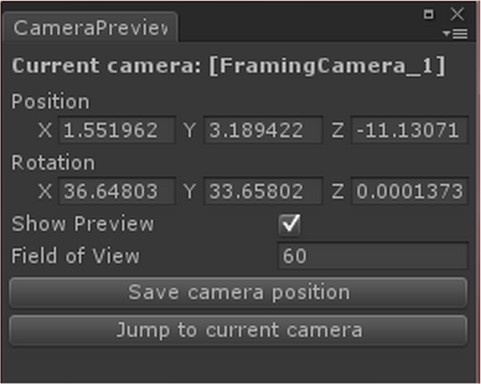
\includegraphics[width=0.60\textwidth]{Pics/Dummy} % Højre billede
\end{minipage} \\ % Captions og labels
\begin{minipage}[t]{0.45\textwidth}
\caption{Caption text for left picture.} % Venstre caption og label
\label{fig:cap1}
\end{minipage} \hfill
\begin{minipage}[t]{0.45\textwidth}
\caption{Caption text for right picture} % Højre caption og label
\label{fig:cap2}
\end{minipage}
\end{figure}

%%% ---------- This is how to make a source reference ---------- %%%
According to bla bla \cite{haigh-hutchinson_real-time_2009} %% passive source
at cite flere: \cite{haigh-hutchinson_real-time_2009, haigh-hutchinson_real-time_2009, haigh-hutchinson_real-time_2009}


%%% ---------- This is how to make bullet points ---------- %%%
\begin{itemize}
\item \textbf{Wavelenght} - Measured in meters from wave top to wave top and denoted as $\lambda$.
\item \textbf{Frequency} - Measured in oscillations per second, Hz, denoted $f$.
\item \textbf{Energy} - Measured in electronvolts, eV, denoted $E$.
\end{itemize}

%%% ---------- This is how to do math stuff ---------- %%%
To derive the wavelength or the frequency, formula \ref{eq:wavelenght} is applied:
\begin{align}
\centering 
\lambda = \frac{C}{f}
\label{eq:wavelenght} 
\end{align}
where {$C$} is the speed of light.



%%% This is how to make footnotes %%%
Hello, I need a footnote \footnote[0]{You can read me, no?}.

%%% This is how to insert a table %%%
\begin{table}[htbp]
\centering
\begin{tabular}{|l|c|c|}
\hline
& Personer
& Totalpris \\\hline
Lasagne
& 4
& 160
\\\hline
Flødekartofler
& 6
& 210
\\\hline
\end{tabular}
\caption{Valg af mad.}
\label{tab:mums}
\end{table} %% GUSTAV'S GUIDE: look at this for how to insert figures, quotes, etc.

%% BONUS STUFF WE MIGHT NEED TO LOOK AT LATER ---------------- VVVVV

%ACKNOWLEDGMENTS are optional
%\section{Acknowledgments}
%This section is optional; it is a location for you
%to acknowledge grants, funding, editing assistance and
%what have you.  In the present case, for example, the
%authors would like to thank Gerald Murray of ACM for
%his help in codifying this \textit{Author's Guide}
%and the \textbf{.cls} and \textbf{.tex} files that it describes.

%
% The following two commands are all you need in the
% initial runs of your .tex file to
% produce the bibliography for the citations in your paper.
\bibliographystyle{abbrv}
\bibliography{references}  % sigproc.bib is the name of the Bibliography in this case
% You must have a proper ".bib" file
%  and remember to run:
% latex bibtex latex latex
% to resolve all references
%
% ACM needs 'a single self-contained file'!
%
%APPENDICES are optional
%\balancecolumns
%\appendix
%Appendix A
%\section{Headings in Appendices}
%The rules about hierarchical headings discussed above for
%the body of the article are different in the appendices.
%In the \textbf{appendix} environment, the command
%\textbf{section} is used to
%indicate the start of each Appendix, with alphabetic order
%designation (i.e. the first is A, the second B, etc.) and
%a title (if you include one).  So, if you need
%hierarchical structure
%\textit{within} an Appendix, start with \textbf{subsection} as the
%highest level. Here is an outline of the body of this
%document in Appendix-appropriate form:
%\subsection{Introduction}
%\subsection{The Body of the Paper}
%\subsubsection{Type Changes and  Special Characters}
%\subsubsection{Math Equations}
%\paragraph{Inline (In-text) Equations}
%\paragraph{Display Equations}
%\subsubsection{Citations}
%\subsubsection{Tables}
%\subsubsection{Figures}
%\subsubsection{Theorem-like Constructs}
%\subsubsection*{A Caveat for the \TeX\ Expert}
%\subsection{Conclusions}
%\subsection{Acknowledgments}
%\subsection{Additional Authors}
%This section is inserted by \LaTeX; you do not insert it.
%You just add the names and information in the
%\texttt{{\char'134}additionalauthors} command at the start
%of the document.
%\subsection{References}
%Generated by bibtex from your ~.bib file.  Run latex,
%then bibtex, then latex twice (to resolve references)
%to create the ~.bbl file.  Insert that ~.bbl file into
%the .tex source file and comment out
%the command \texttt{{\char'134}thebibliography}.
% This next section command marks the start of
% Appendix B, and does not continue the present hierarchy
%\section{More Help for the Hardy}
%The acm\_proc\_article-sp document class file itself is chock-full of succinct
%and helpful comments.  If you consider yourself a moderately
%experienced to expert user of \LaTeX, you may find reading
%it useful but please remember not to change it.
\balancecolumns
% That's all folks!
\end{document}
